%%%%%%%%%%%%%%%%%%%%%%%%%%%%%%%%%%%%%%%%%%%%%%%%%%%%%%%%%%%%%%%%%%%%%%%%
%
%		Chapter 3 - System Models
%
%%%%%%%%%%%%%%%%%%%%%%%%%%%%%%%%%%%%%%%%%%%%%%%%%%%%%%%%%%%%%%%%%%%%%%%%


\begin{topic}[Models of Systems]



\vfil

\begin{center}
\begin{minipage}{300pt}
	\includegraphics*[width=300pt]{images/chap3-xkcd.png}

	\hfill {\footnotesize (image from \href{https://www.xkcd.com/2063/}{xkcd - comic \#2063})}
\end{minipage}
\end{center}


\end{topic}






%%%%%%%%%%%%%%%%%%%%%%%%%%%%%%
%
%  MODULE - Modelling Two Interconnected Quantities
%
%%%%%%%%%%%%%%%%%%%%%%%%%%%%%%



\begin{module}{Modelling Two Quantities}
	\label{sys:model}

	In this module you will learn
\begin{itemize}
	\item how to model two or more inter-dependent quantities using systems
\end{itemize}

\hfill \\


Often, when modelling something, we are faced with two or more quantities that depend on each other. This means that one equation is not enough, so we need to learn how to deal with a system of equations. \\


Just like we did in module \ref{model-odes}, we will follow the step by step procedure developed in chapter 1.

\paragraph{\emph{Step 1.}} Define the problem

\begin{example}
We want to model two interacting populations, like the populations of bears and salmon in a specific natural park.\\

The first step is to decide on what we want to find at the end of the process. 
In this case, we want to know the number of individuals in each population and how they change as time passes. So we define:
\begin{itemize}
	\item $b(t) =$ number of bears in the natural park at time $t$;
	\item $s(t) =$ number of salmon in the natural park at time $t$.
\end{itemize}
\end{example}


\paragraph{\emph{Step 2.}} Build a mind map

\begin{example}
We start with both species in the centre:

\def\SalmonBear{
	\fill[color=orange!50!white] (-4,0) rectangle (-2,1) node[pos=.5] {\color{black}Salmon};
	\fill[color=brown!60!white] (4,0) rectangle (2,1) node[pos=.5] {\color{black}Bear};
}
\begin{center}
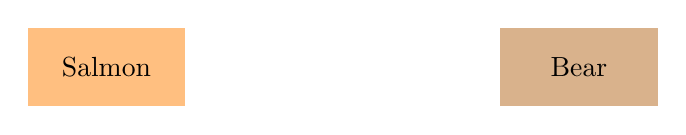
\begin{tikzpicture}
	\SalmonBear
\end{tikzpicture}
\end{center}

We can start brainstorming about the things that affect these populations:
\begin{center}
%\begin{tikzpicture}
%	\SalmonBear
%    \begin{scope}[decoration={
%    markings,
%    mark=at position 0.5 with {\arrow{>}}}
%    ]
%	\draw[postaction={decorate}] (-2,1) arc (120:60:4) node[pos=0.5,above] {food};
%    \draw[postaction={decorate}] (2,0) arc (300:240:4) node[pos=0.5,below] {hunts};
%    \end{scope}
%    \draw (-3,0) -- (-4,-1);
%    \fill[color=green!50!white] (-5.25,-2) rectangle (-2.75,-1) node[pos=.5] {\color{black}reproduction};
%    \draw (-3,1) -- (-4,2);
%    \fill[color=yellow!50!white] (-5.25,2) rectangle (-2.75,3) node[pos=.5] {\color{black}habitat limits};
%    \draw (3,0) -- (4,-1);
%    \fill[color=red!50!white] (5.25,-2) rectangle (2.75,-1) node[pos=.5] {\color{black}competition};
%    \draw (3,1) -- (4,2);
%    \fill[color=yellow!50!white] (5.25,2) rectangle (2.75,3) node[pos=.5] {\color{black}habitat limits};
%\end{tikzpicture}
\begin{tikzpicture}
	\SalmonBear
    \begin{scope}[decoration={
    markings,
    mark=at position 0.5 with {\arrow{>}}}
    ]
    \draw[postaction={decorate}] (-2,0.5) -- (2,0.5) node[pos=0.5,above] {food};
    \draw[postaction={decorate}] (2,0) arc (300:240:4) node[pos=0.5,below] {hunts};
    \end{scope}
    \draw (-3,0) -- (-4,-1);
    \fill[color=green!50!white] (-5.25,-2) rectangle (-2.75,-1) node[pos=.5] {\color{black}reproduction};
    \draw (-3,1) -- (-0.5,2);
    \draw (3,1) -- (0.5,2);
    \fill[color=yellow!50!white] (-1.5,2) rectangle (1.5,3) node[pos=.5] {\color{black}habitat limits};
    \draw (3,0) -- (4,-1);
    \fill[color=red!50!white] (5.25,-2) rectangle (2.75,-1) node[pos=.5] {\color{black}competition};
\end{tikzpicture}
\end{center}
	
\end{example}


\paragraph{\emph{Step 3.}} Make assumptions

\begin{example}
In this step, we discuss which of the boxes in the mind map we want to actually consider in our model, and which assumptions we need to make to consider them. \\

Let us start with how these species interact with each other:
\begin{enumerate}
	\item Salmon provide food for bears: the bear population profits from each encounter with salmon. How does each bear-salmon encounter affect the bear population?
	\item Bears hunt salmon: the salmon population is likely to decrease with each encounter with a bear. How does each bear-salmon encounter affect the salmon population?
\end{enumerate}

These two components are essential in our model, so we need to include them. It still leaves some freedom on how to do this. \\

There are other elements that we might want to include in our model:
\begin{enumerate}[start=3]
	\item Salmon reproduction: in the absence of predators and under ideal conditions, salmon should grow according to the Malthusian model, i.e. the rate of growth is proportional to the number of salmon;
	\item Bear competition: bears are mainly predators, so without salmon, their numbers will decrease, also according to the Malthusian model;
	\item Habitat limits: these species live in habitats that have limited resources, so we can consider a carrying capacity for each species.
\end{enumerate}

To make the model simpler, we will \emph{ignore habitat limits}. This means that this model will not be accurate if the populations become very large.
	
\end{example}


\paragraph{\emph{Step 4.}} Construct a model

\begin{example}
We will start with our populations:
\begin{itemize}
	\item $b(t)$
	\item $s(t)$
\end{itemize}
and we will start adding components to each of these one by one. \\

For the first two items, we need to estimate the number of encounters salmon-bear. We assume that the number of encounters is proportional to the number of all possible encounters: \emph{$b(t)\, s(t)$}.

\begin{enumerate}
	\item Salmon provide food for bears: for every possible salmon-bear encounter, there is a probability that a bear actually encounters a salmon, and then there is a chance that the bear will catch the salmon. Each catch improves the possibility that the bear population will increase. All these put together means that this factor should increase the bear growth rate by \emph{$a \,b(t)\, s(t)$}, where the constant $a$ needs to be found.
	\item Bears hunt salmon: similarly to the previous item, for every possible encounter, there is a probability that the bear actually encounters a salmon, and then there is a chance that the bear will catch the salmon. Every catch will decrease the salmon population, so the salmon growth rate will decrease by \emph{$c \,b(t) \,s(t)$}, there the constant $c$ needs to be found.
\end{enumerate}

Right now we have the following model:
$$
\begin{cases}
b'(t) = a \,b(t)\, s(t) + \cdots \\
s'(t) = - c \,b(t)\, s(t) + \cdots	
\end{cases}
$$

We continue with the other elements:
\begin{enumerate}[start=3]
	\item Salmon reproduction: this was explained before and should contribute to the salmon growth rate with the term \emph{$d s(t)$}.
	\item Bear competition: this was also explained above and should contribute to the bear growth rate with the term \emph{$-e b(t)$}.
	\item Habitat limits: we decided to ignore this.
\end{enumerate}

We have the model:
$$
\begin{cases}
b'(t) = a \, b(t) \,s(t) -e \, b(t) \\
s'(t) = - c \, b(t) \,s(t) + d \, s(t)
\end{cases}
$$

To find the constants $a,c,d,e$, we would probably need to go back to Step 3 and make further assumptions related to the way that we are measuring them.
\end{example}



\paragraph{\emph{Step 5.}} Model assessment

\begin{example}

We can do several things here. 

One of the things that we can do is approximate its solutions using Euler's Method discussed in Module \ref{Approximation}. 

Let us assume, for this example the constants: $a=1$, $e=10$, $c=1$, $d=5$ and a time step $\Delta t = 0.5$ and we assumed an initial population of $b(0)=6$ and $s(0)=9$. Then we obtain the graph below:


\begin{center}
\includegraphics*[width=200pt]{images/module16-lotka-volterra.png}
\end{center}
\begin{itemize}
	\item \url{https://www.desmos.com/calculator/zywspwstwk} \hfill \qrcode{https://www.desmos.com/calculator/zywspwstwk}
\end{itemize}

The $x-$axis is the bear population while the $y-$axis is the salmon population. Each dot gives an approximation of the populations $\Delta t = 0.5$ time units after the previous approximation.\\


From this approximation, we can say infer that this model creates a population cycle, but it seems to spiral outwards: 
\begin{center}
\includegraphics*[width=200pt]{images/module16-lotka-volterra-more.png}
\end{center}

\begin{itemize}
	\item Is having a population cycle a feature that our model should have?
	\item Is the spiralling outwards a feature we want in our model?
	\item Is the spiralling a feature of the model or the approximation? If it's from the approximation, how does the model behave?
\end{itemize}

I'll let you brainstorm and think of other ways you can assess this model.
\end{example}

\begin{graybox}
There are lots of other tools to create slope fields and approximate solutions of systems of ODEs.

\begin{itemize}
	\item GeoGebra approximation of the same model, called the Lotka-Volterra model:
	
	\hfill \qrvideo{https://www.geogebra.org/m/KqNV7eHB}
	
	\item WolframAlpha slope field of the same model:

	\hfill \qrvideo{https://uoft.me/modelling-sys-wa}

	\item WolframAlpha stream plot of the same model:

	\hfill \qrvideo{https://uoft.me/modelling-sys-wa2}
	
	\item There are also better methods of approximating ODEs and systems, e.g. \href{https://en.wikipedia.org/wiki/Runge-Kutta_methods}{Runge-Kutta methods} 
	
	\hfill \qrvideo{https://en.wikipedia.org/wiki/Runge-Kutta_methods}
\end{itemize}

\end{graybox}


%\paragraph{\emph{Step 6.}} Putting it all together in a report
%
%We'll skip this part here.
%




	\begin{exercises}

	\begin{problist}
	
	\prob Create a model for two cooperating populations, like sharks and remoras. 
	
	
%	\begin{center}
%		\includegraphics*[height=150pt]{images/module15-spring-mass-dashpot.pdf}
%	\end{center}
	
	
	\begin{minipage}{.35\textwidth}
		\prob We have a spring attached to a mass and with a dashpot. 
		\begin{enumerate}
			\item Model the position of the mass as time changes.
			\item Obtain a system of two first-order ODEs. Remember to explain how the new functions relate to the spring-mass-dashpot system.
		\end{enumerate}
	\end{minipage}
	\hfill
	\begin{minipage}{100pt}
		\includegraphics*[height=100pt]{images/module16-spring-mass-dashpot.pdf}
	\end{minipage}

	\prob Model a vehicle with a special engine that provides an acceleration to the car proportional to the fuel left.
	
	\prob Imagine two twin babies and model their crying volume. Assume that they naturally become tired and stop crying if alone, but they cry more if the other twin is crying.
	
	
	
	\begin{minipage}{.35\textwidth}
		\prob Create a simplified model for a tree, considering the height of the tree and its leaf area and how they affect each other.	
	\end{minipage}
	\hfill
	\begin{minipage}{100pt}
		\includegraphics*[height=100pt]{images/module16-tree.pdf}
	\end{minipage}

	\prob Create a model on how a student's confidence in her own ability affects her learning/knowledge of a subject. Remember the Ebbinghaus' ``forgetting curve''.

	\begin{center}
		\includegraphics*[width=125pt]{images/module16-UofT2YYZ.pdf}	
	\end{center}

	\prob Imagine that there are two ways to travel from UofT to Toronto's Pearson airport (YYZ). Both paths take the same time if there is no traffic. You want to direct people on the fastest path. Create a model for choosing the fastest path.
	
	
	\prob Create a model for the sales of a specific brand of sneakers. The goal is to capture the influence of famous people and non-famous people on each other's purchases.
	
	\prob Create a model on how the population and the cost of living in Toronto affect each other.
	
	
	\end{problist}
\end{exercises}

\end{module}



\begin{lesson}
	\Title{Modelling Two Quantities}

	\Heading{Objectives}
	\begin{itemize}
		\item Bla
	\end{itemize}
	
	\Heading{Motivation} 

\end{lesson}




\question We want to model two competing populations, like cheetahs and lions: they don't hunt each other, but they hunt the same prey.
\begin{parts}
	\item Create a model for these two populations.
	\item Using Desmos or WolframAlpha, create a slope field in the plane where the horizontal axis is one population and the vertical one is the other.
	\item Using the slope field, deduce some properties of your model and discuss how closely it matches what you expect from these populations.

	\item Extend the model to include a population of antelopes.	
\end{parts}





\bookonlynewpage


\question
	A cheetah is chasing an antelope. We want a model of their positions as they run.
	
	
\begin{annotation}
	\begin{goals}
		This exercise is not required to do in lecture.
		
		Allow some brainstorming and try to create a structure for this problem:
		\begin{itemize}
			\item Positions seen from above ($xy-$plane).
			\item Only need $x_a(t), y_a(t)$ and $x_c(t), y_c(t)$
			\item Focus on the cheetah: where is she heading to?
			\item For the antelope, students need to come up with an escape strategy
			\item Model will be nonlinear!
		\end{itemize}
	\end{goals}
\end{annotation}




\standardonlynewpage

%%%%%%%%%%%%%%%%%%%%%%%%%%%%%%
%
%  MODULE - Solving Systems
%
%%%%%%%%%%%%%%%%%%%%%%%%%%%%%%



\begin{module}{Systems of two linear ODEs with constant coefficients}
	\label{sys:solve}

	In this module you will learn
\begin{itemize}
	\item how to solve systems of two linear first-order ODEs with constant coefficients
\end{itemize}

\hfill \\


First, a system of two first-order ODEs has the form:
$$
\begin{cases}
x'(t) = f\big(t, x(t),y(t)\big) \\	
y'(t) = g\big(t, x(t),y(t)\big)
\end{cases}
$$
where the functions $f$ and $g$ are continuous and have continuous derivatives. \\

This system could be nonlinear, so we are only considering linear systems with constant coefficients, which means that they have a very specific form:
$$
\begin{cases}
	x'(t) = a x(t) + b y(t) + e\\
	y'(t) = c x(t) + d y(t) + f
\end{cases}
%
\quad \Leftrightarrow \quad 
	\begin{bmatrix} x'(t) \\ y'(t) \end{bmatrix}
	=
	\begin{bmatrix} a & b \\ c & d \end{bmatrix}
	\begin{bmatrix} x(t) \\ y(t) \end{bmatrix}
	+	\begin{bmatrix} e \\ f \end{bmatrix}
%
\quad \Leftrightarrow \quad 
	\vec{r}'(t)
	=
	A \, \vec{r}(t) + \vec{b}
$$
where
$$
\vec{r}(t) = \begin{bmatrix} x(t) \\ y(t) \end{bmatrix}
\quad , \quad 
A = \begin{bmatrix} a & b \\ c & d \end{bmatrix}
\quad and \quad 
\vec{b}=\begin{bmatrix} e \\ f \end{bmatrix}.
$$

The unknown functions we are trying to find is $\vec{r}(t)$. \\


\paragraph{\emph{Homogeneous Systems.}} These are systems of the form above with $\vec{b} = \vec{0}$.

This means that we want to find all functions $\vec{r}(t)$ that satisfy
$$
\vec{r}'(t) = A \vec{r}(t).
$$


\begin{example}
Let us start with an example of the same problem where $\vec{r}(t)$ is a ``one-dimensional'' vector, a scalar function $u(t)$, and the matrix $A$ is a ``one-dimensional matrix'', a constant $a$. \\

We want to solve the problem	
$$
u'(t) = a \cdot u(t).
$$

We have seen how to solve these kind of problems before. The solutions are
$$
u(t) = c e^{at},
$$
where $c$ can be any constant.
\end{example}

In our two-dimensional case, it is a little more complicated. We can't just write $e^{At}$ where $A$ is a matrix (this expression can make sense, but we would have to find out what is the exponential of a matrix). \\

So we can use the example above to make an \emph{educated guess}: the solution should look like an exponential:
$$
\vec{r}(t) = 
\vec{c} \, e^{\lambda t},
$$
where $\vec{c}$ is a constant vector. \\

If our guess is correct, to find $\vec{r}(t)$, we only need to find $\lambda$ and $\vec{c}$. \\

Let us see what happens when we use this guess and plug it into the system of ODEs:
\begin{align*}
\vec{r}'(t) = A \vec{r}(t) \quad
	& \Leftrightarrow \quad \vec{c} \lambda e^{\lambda t} = A \vec{c} e^{\lambda t} \\
	& \Leftrightarrow \quad \vec{c} \lambda = A \vec{c}.
\end{align*}

This is a problem you have seen before -- and eigenvalue-eigenvector problem: 
\begin{itemize}
	\item $\lambda$ can be any eigenvalue of the matrix $A$
	\item $\vec{c}$ can be any eigenvector of $A$ associated with $\lambda$ 
\end{itemize}

This means that we might have multiple choices for eigenvalues and eigenvectors, or even that eigenvalues and eigenvectors involve complex numbers.
Let us split our study of possible solutions in three cases.



%%%%%%%%%       %%%%%%%%%       %%%%%%%%%       %%%%%%%%%       %%%%%%%%%

\subsection{Two real and distinct eigenvalues}

\begin{example}
Consider the problem
$$
\vec{r}'(t) = \begin{bmatrix}	
 10 & 18 \\ -6 & -11	
 \end{bmatrix} \, \vec{r}(t).
$$

Then, the eigenvalues and eigenvectors of the matrix are
\begin{itemize}
	\item $\lambda_1=-2$ with eigenvector $\vec{v}_1 = \begin{bmatrix} 3 \\ -2 \end{bmatrix}$
	\item $\lambda_2=1$ with eigenvector $\vec{v}_2 = \begin{bmatrix} 2 \\ -1 \end{bmatrix}$
\end{itemize}

This means that we found two solutions:
$$
\vec{r}_1(t) = \begin{bmatrix} 3 \\ -2 \end{bmatrix} e^{-2t}
\quad \text{ and } \quad \vec{r_2}(t) = \begin{bmatrix} 2 \\ -1 \end{bmatrix} e^{t}.
$$

Then, we can show that 
$$
\vec{r}(t) = c_1 \begin{bmatrix} 3 \\ -2 \end{bmatrix} e^{-2t}
+c_2\begin{bmatrix} 2 \\ -1 \end{bmatrix} e^{t}
$$
is also a solution of the problem for any constants $c_1$ and $c_2$.

In fact, we can show that this formula captures all possible solutions for this problem.
\end{example}


\begin{video}
	\begin{itemize}
		\item \qrvideo{https://youtu.be/YUjdyKhWt6E}
	\end{itemize}
\end{video}




%%%%%%%%%       %%%%%%%%%       %%%%%%%%%       %%%%%%%%%       %%%%%%%%%

\subsection{Two complex eigenvalues}

We actually don't need to know a lot about complex numbers to be able to understand how to solve this case.
The results about complex values that are necessary to know will be included in the box below.

\begin{definition}[Complex numbers]
\begin{itemize}
	\item A complex number is a number of the form $z=a+ib$ where $i$ is called the imaginary constant and satisfies $i^2=-1$.
	\item Given a complex number $z=a+ib$, we call $\overline{z}=a-ib$ its complex conjugate. It satisfies:
	$$ z \cdot \overline{z} = a^2+b^2 = |z|^2.$$

	\item If a matrix has real components and two complex eigenvalues, then the eigenvalues are complex conjugates of each other. Moreover, the eigenvectors are also complex conjugates of each other.
	\item Euler's Formula: $e^{i \theta} = \cos(\theta) + i \sin (\theta)$.
\end{itemize}
\end{definition}




\begin{example}
Consider the problem
$$
\vec{r}'(t) = \begin{bmatrix}	
 1 & 1 \\ -1 & 1
 \end{bmatrix} \, \vec{r}(t).
$$

Then, the eigenvalues and eigenvectors of the matrix are
\begin{itemize}
	\item $\lambda_1=1+i$ with eigenvector $\vec{v}_1 = \begin{bmatrix} -i \\ 1 \end{bmatrix}$
	\item $\lambda_2=1-i$ with eigenvector $\vec{v}_2 = \begin{bmatrix} i \\ 1 \end{bmatrix}$
\end{itemize}

This means that we found two solutions:
$$
\vec{r}_1(t) = \begin{bmatrix} -i \\ 1 \end{bmatrix} e^{(1+i)t}
\quad \text{ and } \quad \vec{r}_2(t) = \begin{bmatrix} i \\ 1 \end{bmatrix} e^{(1-i)t}.
$$

Then, all solutions of this system of ODEs can be expressed as
$$
\vec{r}(t) = c_1 \begin{bmatrix} -i \\ 1 \end{bmatrix} e^{(1+i)t}
+c_2\begin{bmatrix} i \\ 1 \end{bmatrix} e^{(1-i)t}.
$$

There is a problem with the form of these solutions: they involve complex numbers!

Imagine that we start with a problem where we have two (real) quantities that interact with each other through this system of differential equations.
Then we expect these quantities to measure in real numbers, not complex.

\begin{itemize}
	\item This means that we expect \emph{the imaginary part of this solutions to cancel out}.
\end{itemize}

So let us manipulate this formula using Euler's formula and see if we can re-write in such a way that doesn't involve complex numbers. \\

We have:
\begin{align*}
	e^{(1+i)t} &= e^t \cdot e^{it} = e^t \big( \cos(t) + i \sin(t)\big) \\
	e^{(1-i)t} &= e^t \cdot e^{-it} = e^t \big( \cos(t) - i \sin(t)\big)
\end{align*}

So our solution expands to:
$$
\vec{r}(t) = c_1 \begin{bmatrix} -i \\ 1 \end{bmatrix} e^t \big( \cos(t) + i \sin(t)\big)
+c_2\begin{bmatrix} i \\ 1 \end{bmatrix} e^t \big( \cos(t) - i \sin(t)\big).
$$

We can now manipulate this expression:
\begin{align*}
\vec{r}(t) 
	& = e^t
		\begin{bmatrix}
			-i c_1 	\big( \cos(t) + i \sin(t)\big) + i c_2 \big( \cos(t) - i \sin(t)\big) \\
			c_1 	\big( \cos(t) + i \sin(t)\big) + c_2 \big( \cos(t) - i \sin(t)\big) \\
		\end{bmatrix} \\
	& = e^t 
		\begin{bmatrix}
			(c_1+c_2) \sin(t) - i (c_1-c_2) \cos(t) \\
			(c_1+c_2) \cos(t) + i(c_1-c_2) \sin(t)
		\end{bmatrix} \\
	& = e^t \left( (c_1+c_2) \begin{bmatrix} \sin(t) \\ \cos(t) \end{bmatrix}
		+ i (c_1 -c_2) \begin{bmatrix} - \cos(t) \\ \sin(t) \end{bmatrix}
		\right)
\end{align*}

So now we do something that might look like a ``cheating''. We define:
$$
a_1 = c_1+c_2 \quad \text{ and } \quad a_2 = i (c_1-c_2).
$$


Then the solution is
$$
\vec{r}(t) = a_1\begin{bmatrix} \sin(t) \\ \cos(t) \end{bmatrix} e^t
		+ a_2 \begin{bmatrix} - \cos(t) \\ \sin(t) \end{bmatrix} e^t.
$$

This last form doesn't include any complex numbers and is equivalent to the previous form.

\end{example}

\begin{graybox}
	It may look like the final solution above still includes complex numbers in the constants $a_1$ and $a_2$. 
	
	To convince yourself that this is not the case, solve the following exercise.\\
	
	Find the unique solution of
	$$
	\vec{r}'(t) = \begin{bmatrix}	
 		1 & 1 \\ -1 & 1
		\end{bmatrix} 
		\, \vec{r}(t)
	\qquad \text{ with} \qquad
	\vec{r}(0) = \begin{bmatrix}
 			-3 \\ 2
	 \end{bmatrix}
	 $$
	 
	 Find the constants $c_1, c_2$ and then the constants $a_1,a_2$. Which ones are complex and which ones are real?
\end{graybox}

\begin{video}
	\begin{itemize}
		\item \qrvideo{https://youtu.be/TRVS5Wo9LoM}
	\end{itemize}
\end{video}



%%%%%%%%%       %%%%%%%%%       %%%%%%%%%       %%%%%%%%%       %%%%%%%%%

\subsection{One real repeated eigenvalue}


\begin{example}
Consider the problem
$$
\vec{r}'(t) = \begin{bmatrix}	
 5 & 0 \\ 1 & 5	
 \end{bmatrix} \, \vec{r}(t).
$$

Then, there is only one eigenvalue with one eigenvector
\begin{itemize}
	\item $\lambda_1=5$ with eigenvector $\vec{v}_1 = \begin{bmatrix} 0 \\ 1 \end{bmatrix}$, which yield a solution $\vec{r}_1(t) = c_1 \begin{bmatrix} 0 \\ 1 \end{bmatrix} e^{5t}$.
\end{itemize}

This is a \emph{problem} because we need two solutions to put together and obtain two constants, as in the two previous cases.
%\end{example}

\begin{graybox}
To convince yourself that it is a problem, try solving the problem above with initial conditions
$$
\vec{r}(0) = \begin{bmatrix}	0 \\ 4 \end{bmatrix}.
$$

What about with initial conditions
$$
\vec{r}(0) = \begin{bmatrix}	 1 \\ 4 \end{bmatrix} \quad ?
$$
\end{graybox}

%\begin{example}

This means that we ware missing one solution -- that will enable us to solve the problem for any initial conditions. \\


Let us re-write the original problem in a different form by letting 
$$
\vec{r}(t) = \begin{bmatrix} x(t) \\ y(t)\end{bmatrix}.
$$
Then we have
$$
\begin{cases}
x'(t) = 5 x(t) \\
y'(t) = x(t) +5 y(t)	
\end{cases}
$$
These are two ODEs, but we can solve the first and then tackle the second one.
We obtain
$$
\begin{cases}
	x(t) = c_2 e^{5t} \\
	y(t) = 	c_1 e^{5t} + c_2 t e^{5t} 
\end{cases}
\quad \Leftrightarrow \quad
	\vec{r}(t) = \begin{bmatrix}
		c_2 \\ c_1 + c_2 t
	\end{bmatrix} e^{5t}
\quad \Leftrightarrow \quad
	\vec{r}(t) = c_1 \begin{bmatrix} 0 \\ 1 \end{bmatrix} e^{5t} + c_2
	\begin{bmatrix}	1 \\ t
	\end{bmatrix} e^{5t}
$$
\end{example}

\begin{graybox}
Observe that the solution we found has the form:
$$
	\vec{r}(t) = \underbrace{c_1 \begin{bmatrix} 0 \\ 1 \end{bmatrix} e^{5t}}_{\text{solution } \vec{r}_1(t)} + c_2 \left( 
	\underbrace{\begin{bmatrix}	1 \\ 0 \end{bmatrix}}_{\text{new vector } \vec{w}} e^{5t} + \underbrace{\begin{bmatrix} 0  \\ 1 
	\end{bmatrix}}_{\vec{v}_1} t e^{5t}\right).
$$

So we can make another \emph{educated guess} that the solution we were missing has the form:
$$
\vec{r}_2(t) = \left(\vec{w} + \vec{v}_1 t\right) e^{\lambda t}.
$$

With this form in mind, we can plug it into the system of ODEs \quad $\vec{r}'(t) = A \vec{r}(t)$ \quad, which has exactly one eigenvalue $\lambda$, to get:
$$
\lambda \vec{w}e^{\lambda t} + \lambda \vec{v}_1 t e^{\lambda t} + \vec{v}_1 e^{\lambda t}
= A \vec{w} e^{\lambda t} + A \vec{v}_1 t  e^{\lambda t}
$$
which is equivalent to:
$$
\lambda \vec{w} + \underbrace{\lambda \vec{v}_1}_{=A \vec{v}_1} t  + \vec{v}_1
= A \vec{w}  + A \vec{v}_1 t 
	\quad \Leftrightarrow \quad
	\left( \lambda I - A \right ) \vec{w} = \vec{v}_1
$$
%which becomes
%$$
%\lambda \vec{w} + \vec{v}_1
%= A \vec{w}  
%	\quad \Leftrightarrow \quad
%	\left( \lambda I - A \right ) \vec{w} = \vec{v}_1
%$$

Since at this point we already know $\lambda$ and $\vec{v}_1$, we can now find $\vec{w}$ in a similar way used to find the eigenvector $\vec{v}_1$. The vector $\vec{w}$ is called a \emph{generalized eigenvector} of $A$ associated with the eigenvalue $\lambda$.

\end{graybox}

\begin{video}
	\begin{itemize}
		\item \qrvideo{https://youtu.be/hCShTLmeZN4}
	\end{itemize}
\end{video}






	\begin{exercises}

	\begin{problist}
	\prob \label{mod17-gensol}Find the general solution of the problem $\vec{r}'(t) = A \vec{r}(t)$ for the following matrices:
	\begin{enumerate}
	\begin{minipage}{.2\textwidth}
		\item $A = \begin{bmatrix} -7 & 6 \\ -9 & 8 \end{bmatrix}$;
		\item $A = \begin{bmatrix} 22 & 24 \\ -15 & -16\end{bmatrix}$;
		\item $A = \begin{bmatrix} 0 & 1 \\ -5 & 0 \end{bmatrix}$;
		\item $A = \begin{bmatrix} 0 & 1 \\ 5 & 0 \end{bmatrix}$;
		\item $A = \begin{bmatrix} 1 & \sqrt{3} \\ \sqrt{3} & -1\end{bmatrix}$;
		\item $A = \begin{bmatrix} 1 & \sqrt{3} \\ -\sqrt{3} & 1\end{bmatrix}$;
	\end{minipage}
	\qquad
	\begin{minipage}{.2\textwidth}
		\item $A = \begin{bmatrix} 0 & 1 \\ -4 & -4 \end{bmatrix}$;
		\item $A = \begin{bmatrix} -4 & -6 \\ 2 & 3 \end{bmatrix}$;
		\item $A = \begin{bmatrix} 2 & -3 \\ 0 & 2 \end{bmatrix}$;
		\item $A = \begin{bmatrix} 2 & 0 \\ 0 & 2 \end{bmatrix}$;
		\item $A = \begin{bmatrix} 0 & 0 \\ 1 & 0\end{bmatrix}$; 
		\item $A = \begin{bmatrix} 0 & 0 \\ 0 & 1\end{bmatrix}$; 
	\end{minipage}
	\end{enumerate}

	\prob For each of the problems in the previous exercise, find the solution that satisfies the initial conditions:
	\begin{enumerate}[label=(\roman*)]
		\item $\vec{r}(0)=\begin{bmatrix} 0 \\ 0 \end{bmatrix}$;
		\item $\vec{r}(0)=\begin{bmatrix} 1 \\ 3 \end{bmatrix}$;
		\item $\vec{r}(1)=\begin{bmatrix} -2 \\ 2 \end{bmatrix}$.
	\end{enumerate}


	\prob Consider the problem $\vec{r}'(t) = \begin{bmatrix} 2 & 0 \\ 1 & 3 \end{bmatrix} \vec{r}(t) + \begin{bmatrix} -2 \\ 11 \end{bmatrix}$.
	\begin{enumerate}
		\item Show that $\vec{e}(t) = \begin{bmatrix} 1 \\ -4 	\end{bmatrix}$ is a solution of this problem.
		\item Find the general solution of 
		$$\vec{u}'(t) = \begin{bmatrix} 2 & 0 \\ 1 & 3 \end{bmatrix} \vec{u}(t).$$
		\item Let $\vec{r}(t) = \vec{u}(t) + \vec{e}(t)$. Show that this is a solution of the original problem.
		\item Let $\vec{r}_1(t)$ and $\vec{r}_2(t)$ be two solutions of the original problem. 
		\begin{enumerate}
			\item Is $\vec{r}_1(t) + \vec{r_2}(t)$ a solution? 
			\item Is $3\vec{r}_1(t) $ a solution? 
			\item Write a result on how one can safely combine solutions of non-homogeneous problems.
		\end{enumerate}
	\end{enumerate}

	
	\prob \label{prob:sys-nonhomogeneous}Consider the problem  \quad $\vec{r}'(t) = \begin{bmatrix} 1 & 2 \\ 3 & 0 \end{bmatrix}
 \vec{r}(t)+\begin{bmatrix} -5 \\ 3 \end{bmatrix}
$.
	\begin{enumerate}
		\item Observe that this system is an autonomous system of ODEs. What is the equilibrium solution? 
		\item Let the equilibrium solution solution you just found be called $\vec{e}$. Consider $\vec{u}(t) = \vec{r}(t) - \vec{e}$, where $\vec{r}(t)$ is the solution of the original problem. Show that 
			$$ \vec{u}'(t) = A \, \vec{u}(t).$$
		\item Find $\vec{u}(t)$.
		\item Find $\vec{r}(t)$.
		\item Write a procedure to solve any problem of the form
			$$ \vec{r}(t) = A \, \vec{r}(t) + \vec{b}. $$
	\end{enumerate}
	
	
	\prob \label{prob:sys-superposition}Consider the problem \quad $\vec{r}'(t) = A \, \vec{r}(t)$.
	Assume that we have two solutions $\vec{r_1}(t)$ and $\vec{r_2}(t)$.
	\begin{enumerate}
		\item Show that $\vec{r}(t) = \vec{r_1}(t) + \vec{r_2}(t)$ is a solution also.
		\item Show that $\vec{r}(t) = 2\vec{r_1}(t) - 3\vec{r_2}(t)$ is a solution also.
		\item Find all possible solutions of the problem.
	\end{enumerate}
	
	
		\prob Consider the problem $\vec{r}'(t) = \begin{bmatrix} 1 & -2 \\ -2 & 1 \end{bmatrix} \vec{r}(t)$.
		\begin{enumerate}
			\item Find the solution that satisfies the initial condition $\vec{r}(0)=\begin{bmatrix}1 \\ 0\end{bmatrix}$. Call it $\vec{u}(t)$.
			\item Find the solution that satisfies the initial condition $\vec{r}(0)=\begin{bmatrix}0 \\ 1\end{bmatrix}$. Call it $\vec{v}(t)$.
			\item Define the matrix function
			$$ \Phi(t) = \begin{bmatrix} \vec{u}(t) \; | \; \vec{v}(t) \end{bmatrix} = \begin{bmatrix} u_1(t) & v_1(t) \\ u_2(t) & v_2(t) \end{bmatrix}.$$
			
			Show that $\vec{r}(t) = \Phi(t) \vec{r}_0$ is a solution of the original system of ODEs. Which initial condition does it satisfy?
			
			\item Write a result relating $\Phi(t)$ to the solution of initial-value problems.
			\end{enumerate}

	
	
		\prob \label{mod17:prob-W1}Consider a system of ODEs $\vec{r}'(t) = A \vec{r}(t)$ with two solutions $\vec{r}_1(t)$ and $\vec{r}_2(t)$. 
		
		We want to study the conditions that are necessary on the solutions $\vec{r}_1$ and $\vec{r}_2$ to guarantee that we can solve any initial-value problem.
		
		\begin{enumerate}
			\item What is the general solution for this problem?
			\item If the initial condition is $\vec{r}(0)= \begin{bmatrix} 1 \\ 2 \end{bmatrix}$, then what are the conditions on $\vec{r}_1,\vec{r}_2$ ?
			\item If the initial condition is $\vec{r}(0)= \vec{r_0}$, then what are the conditions on $\vec{r}_1,\vec{r}_2$ ?
		\end{enumerate}

		\prob Consider a system of ODEs $\vec{r}'(t) = A \vec{r}(t)$ with two solutions $\vec{r}_1(t), \vec{r}_2(t)$.
		
			Let $R(t)$ be the matrix 
				$R(t) = \begin{bmatrix} \vec{r}_1(t) & | & \vec{r}_2(t)	\end{bmatrix} $ 
				and let $W(t) = \det R(t)$.
		
		\begin{enumerate}
			\item Show that $W(t)$ is a solution of $W' = (a_{11} + a_{22}) W$.
			\item Solve the ODE above to obtain an expression for $W(t)$.
			\item Show that $W(t)$ is either identically zero, or it's never zero. 
			\item Use this result to simplify your answer to problem \ref{mod17:prob-W1}(c).
		\end{enumerate}
	
	\end{problist}
\end{exercises}

\end{module}



\begin{lesson}
	\Title{Systems of two linear ODEs with constant coefficients}

	\Heading{Objectives}
	\begin{itemize}
		\item Bla
	\end{itemize}
	
	\Heading{Motivation} 

\end{lesson}




\question
Consider a cheetah-lion inspired problem:
$$
\frac{d \,\vec{r}}{dt} = \begin{bmatrix} 3 & -2 \\ -1 & 4\end{bmatrix} \vec{r}.
$$
	
\begin{parts}
	\item Find the two solutions $\vec{r}_1, \vec{r}_2$.
	\item Is $\vec{r}_1(t) + \vec{r}_2(t)$ a solution?
	\item Is $\vec{r}_1(t) - \vec{r}_2(t)$ a solution?
	\item Is $2\vec{r}_1(t) + 3\vec{r}_2(t)$ a solution?
	\item What is the general solution?
	\item Find the solution that satisfies $\vec{r}(0) = \begin{bmatrix} 6 \\ 7\end{bmatrix}$?
\end{parts}


\bookonlynewpage


\question
Consider a problem:
$$
\frac{d \,\vec{r}}{dt} = \begin{bmatrix} 2 & -5 \\ 1 & -2\end{bmatrix} \vec{r}.
$$
	
\begin{parts}
	\item Find the general solution.
	\item Find the solution that satisfies $\vec{r}(0) = \begin{bmatrix} 6 \\ 7\end{bmatrix}$?
\end{parts}




\bookonlynewpage


\question
Consider a problem:
$$
\frac{d \,\vec{r}}{dt} = \begin{bmatrix} 4 & -1 \\ 8 & -2\end{bmatrix} \vec{r} - \begin{bmatrix} 5 \\ 10 \end{bmatrix}.
$$
%[2,3]
\begin{parts}
	\item Find the equilibrium solution.
	\item Find the general solution.
	\item Find the solution that satisfies $\vec{r}(0) = \begin{bmatrix} 2 \\ 3\end{bmatrix}$?
\end{parts}






\standardonlynewpage

%%%%%%%%%%%%%%%%%%%%%%%%%%%%%%
%
%  MODULE - Phase Portraits
%
%%%%%%%%%%%%%%%%%%%%%%%%%%%%%%



\begin{module}{Phase Portraits}
	\label{sys:phase}

	In this module you will learn
\begin{itemize}
	\item how to sketch a phase portrait for a linear system of ODEs with constant coefficients
	\item how to use a phase portrait to deduce properties of solutions
\end{itemize}

\hfill \\

When we solve a system of two ODEs, we obtain two functions $x(t)$ and $y(t)$, so when we want to graph solutions, we have a problem:
\begin{itemize}
	\item Should we sketch each of these functions separately?
	\item Should we sketch them together?
	\item Should we sketch the path as if a particle is moving with coordinates $x(t)$ and $y(t)$?
\end{itemize}

\begin{example}
Consider the initial-value problem
$$
\frac{d\,\vec{r}}{dt} = \begin{bmatrix} 0 & 1 \\ -1 & 0 \end{bmatrix}\vec{r} \quad \text{ with } \quad \vec{r}(0)=\begin{bmatrix} 0 \\ 1 \end{bmatrix},
$$
which has the solution
$$
\vec{r}(t) = \begin{bmatrix}
	\sin(t) \\ \cos(t)
\end{bmatrix}.
$$

Which of the following ways are better?
\begin{itemize}
\item \begin{minipage}{400pt}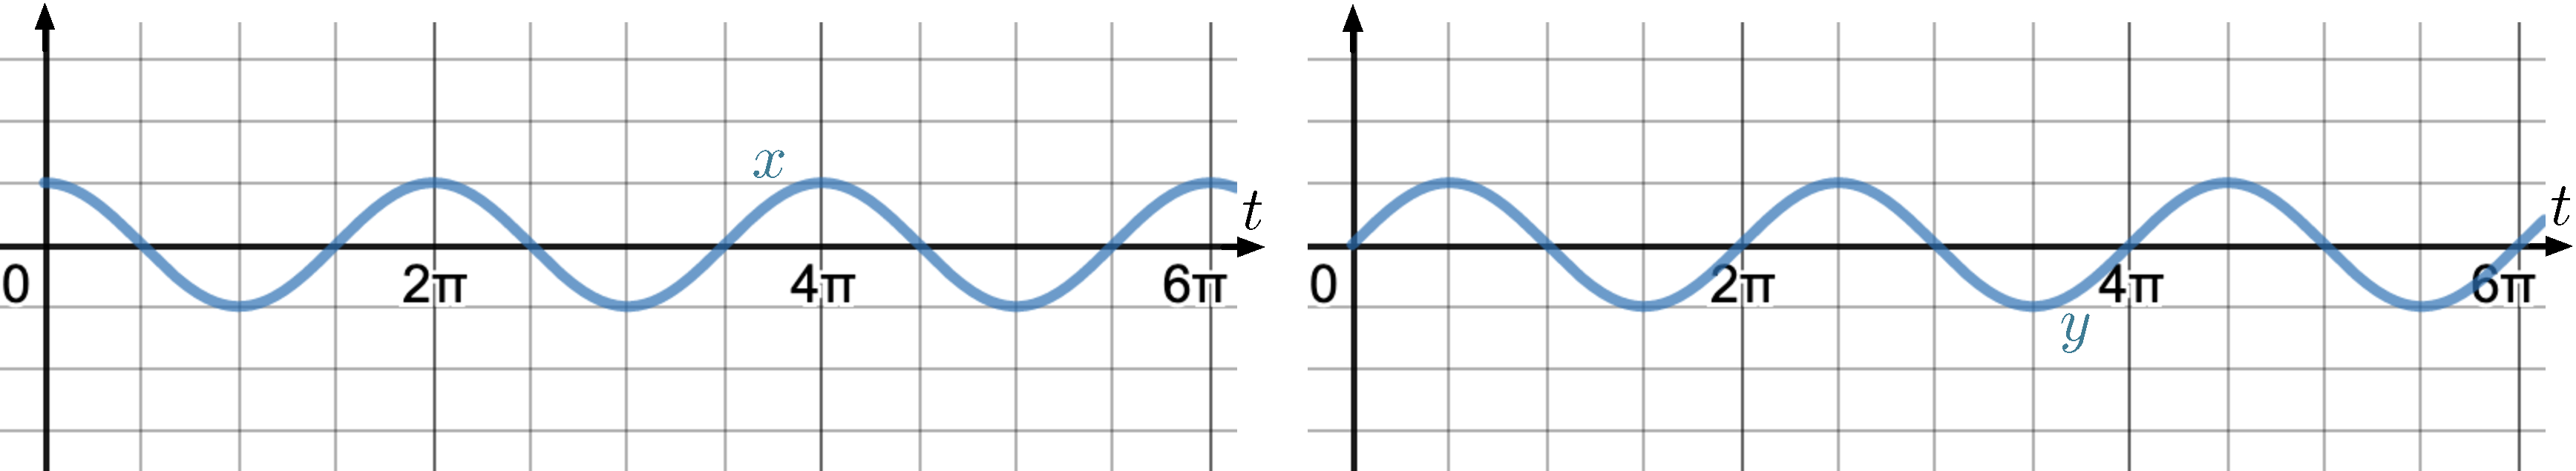
\includegraphics[width=400pt]{images/module18-sep-xy.pdf}\end{minipage}

\item \begin{minipage}{200pt}\includegraphics*[width=200pt]{images/module18-together-xy.pdf}\end{minipage}

\item \begin{minipage}{200pt}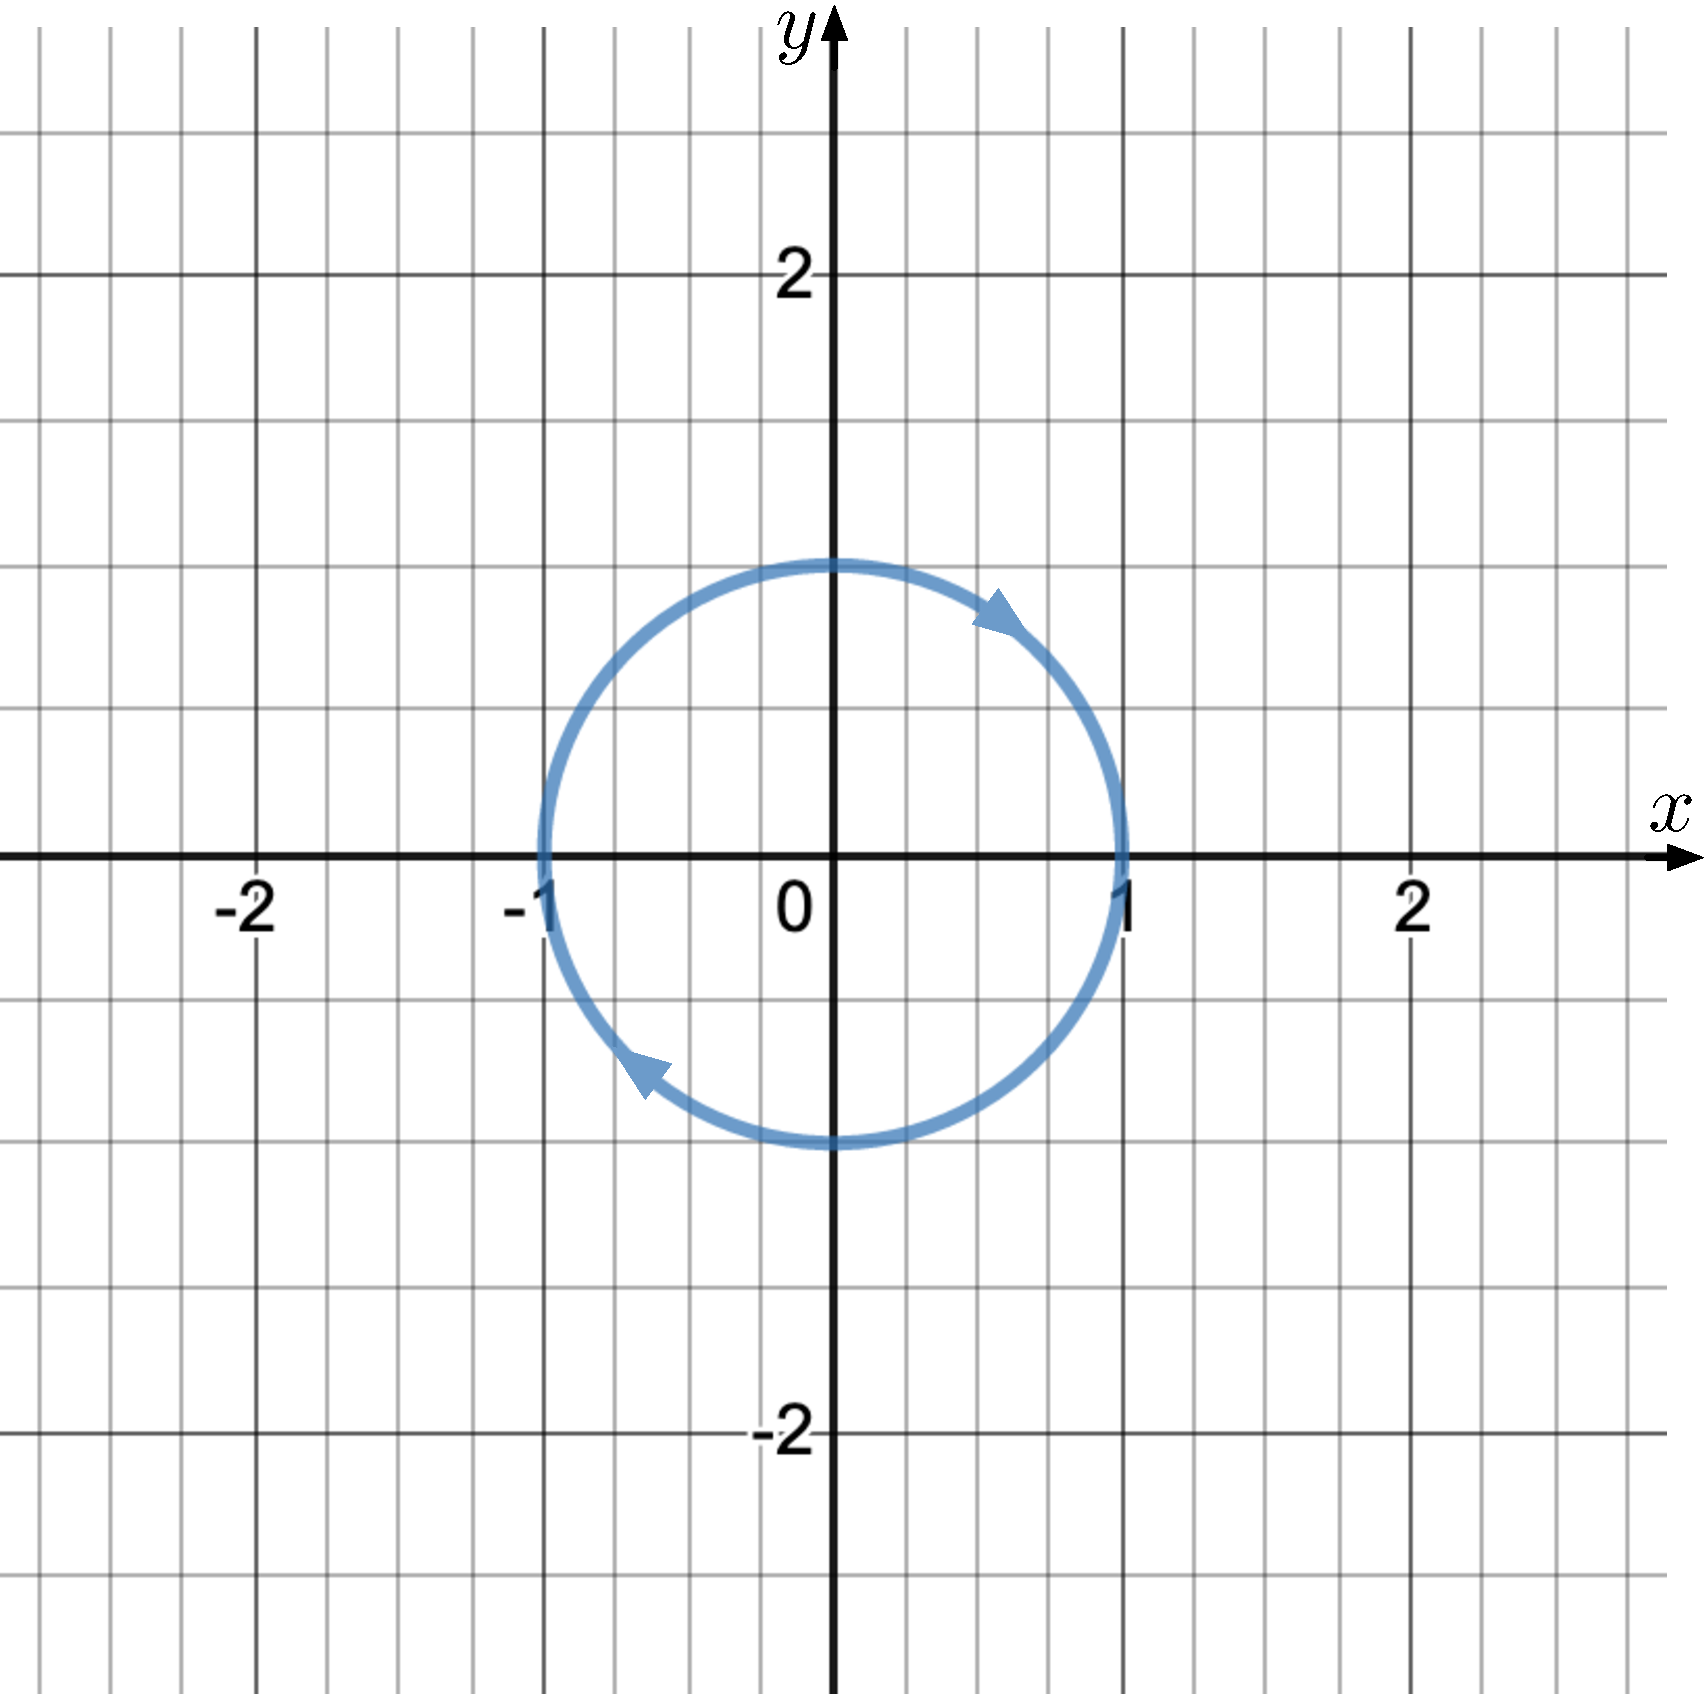
\includegraphics[height=200pt]{images/module18-phaseportrait.pdf}\end{minipage}
\end{itemize}

There is no correct answer, but the last graph gives more information on how the two quantities interact with each other, so we will focus on that type of graph.
\end{example}


The graphs in the example above are graphs of one specific solution. A phase portrait gives an idea of all possible solutions. 
\begin{example}
The last graph of the example is part of which phase portrait?

\begin{center}
\includegraphics*[width=420pt]{images/module18-possiblephaseportraits.pdf}
\end{center}

A phase portrait gives a good idea of how all solutions behave.
\end{example}

Sketching phase portraits for systems of two first-order linear ODEs is important because it gives us insight on how the two components affect each other for all solutions.

\begin{example}
Consider the problem
$$
\frac{d \, \vec{r}}{dt} = \begin{bmatrix} -2 & 3 \\ -3 & -2 \end{bmatrix} \vec{r},
$$
where the matrix $A$ has the eigenvalues and eigenvectors:
\begin{itemize}
	\item Eigenvalues $\lambda_{\pm} = -2 \pm 3i$ with eigenvectors $v_{\pm} = \begin{bmatrix} \mp i \\ 1 \end{bmatrix}$
\end{itemize}

This means that the general solution has the form
\begin{itemize}
	\item $\displaystyle \vec{r}(t) = a_1 \begin{bmatrix} -i \\ 1 \end{bmatrix} e^{(-2+3i)t} + a_2 \begin{bmatrix} i \\ 1 \end{bmatrix} e^{(-2-3i)t}$

	\item[or]
	\item $\displaystyle \vec{r}(t) = c_1 \begin{bmatrix}	 \sin(3t) \\ \cos(3t) \end{bmatrix} e^{-2t} + c_2 \begin{bmatrix}	 -\cos(3t) \\ \sin(3t) \end{bmatrix} e^{-2t}$ \\
\end{itemize}

We can use the general form and start sketching some solutions.

\begin{itemize}
	\item Let $c_1=1$ and $c_2=0$ and we obtain
	$$ \vec{r}(t) = \begin{bmatrix}	 \sin(3t) \\ \cos(3t) \end{bmatrix} e^{-2t}.$$
	
	To sketch this solution, let us start by ignoring the term $e^{-2t}$. 
	
	So we want to sketch $ \vec{r}(t) = \begin{bmatrix}	 \sin(3t) \\ \cos(3t) \end{bmatrix}$:
	\begin{center}
		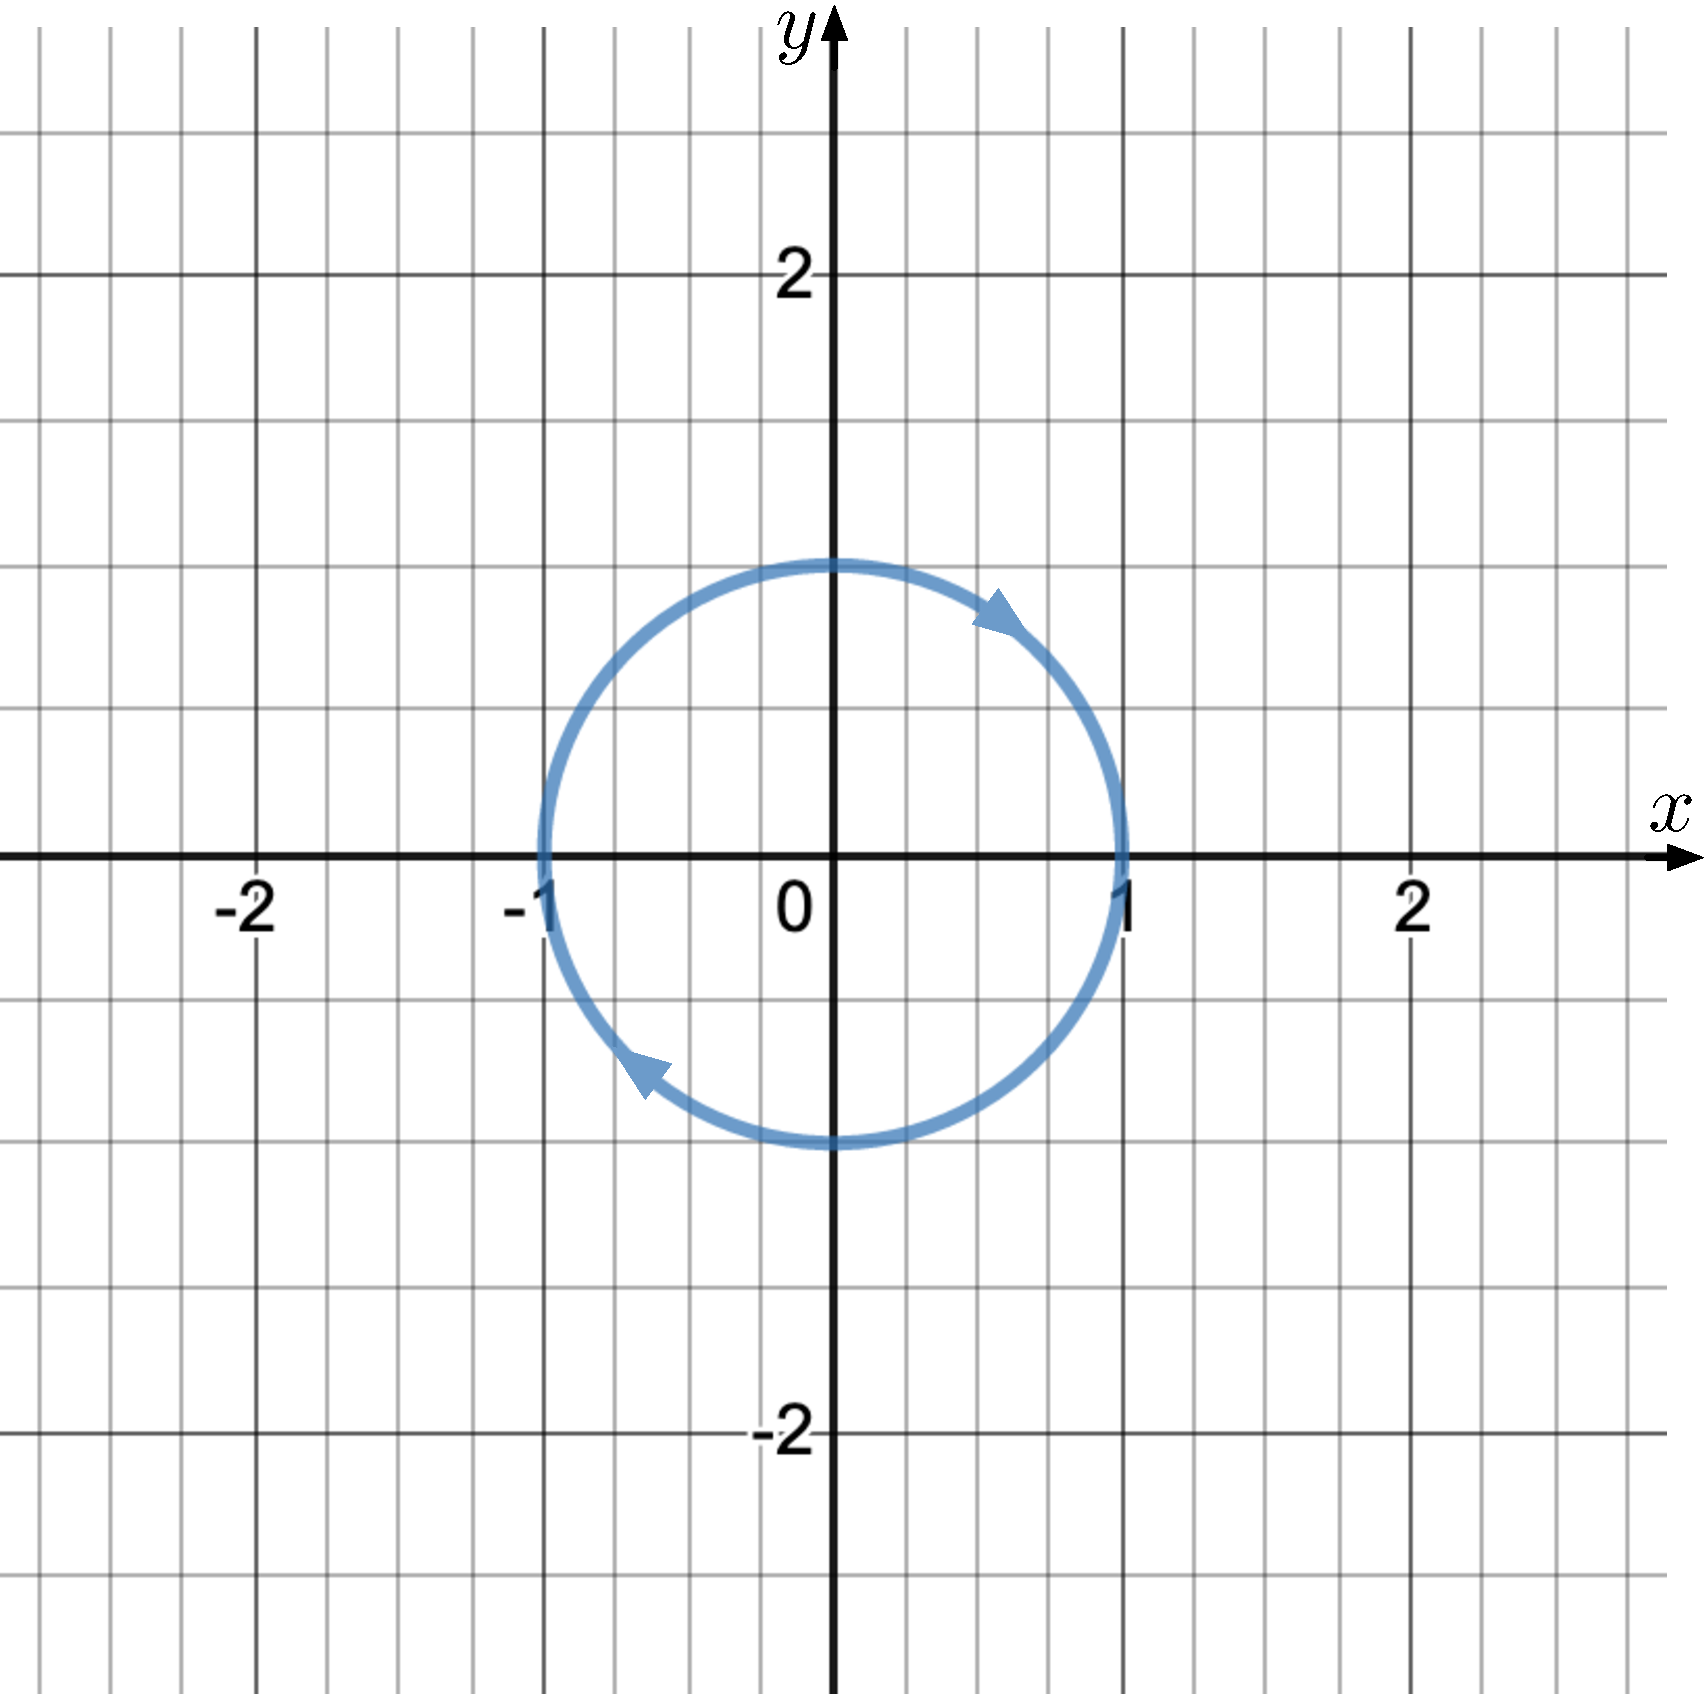
\includegraphics[height=200pt]{images/module18-phaseportrait.pdf}
	\end{center}
	
	The path is going in circles in the clockwise direction.
	
	By multiplying the solution by $e^{-2t}$, which starts at $1$ when $t=0$ and keeps decreasing towards $0$ as $t$ increases, we are creating a graph that keeps revolving around the origin as it converges towards the origin, yielding a spiral.
	\begin{center}
		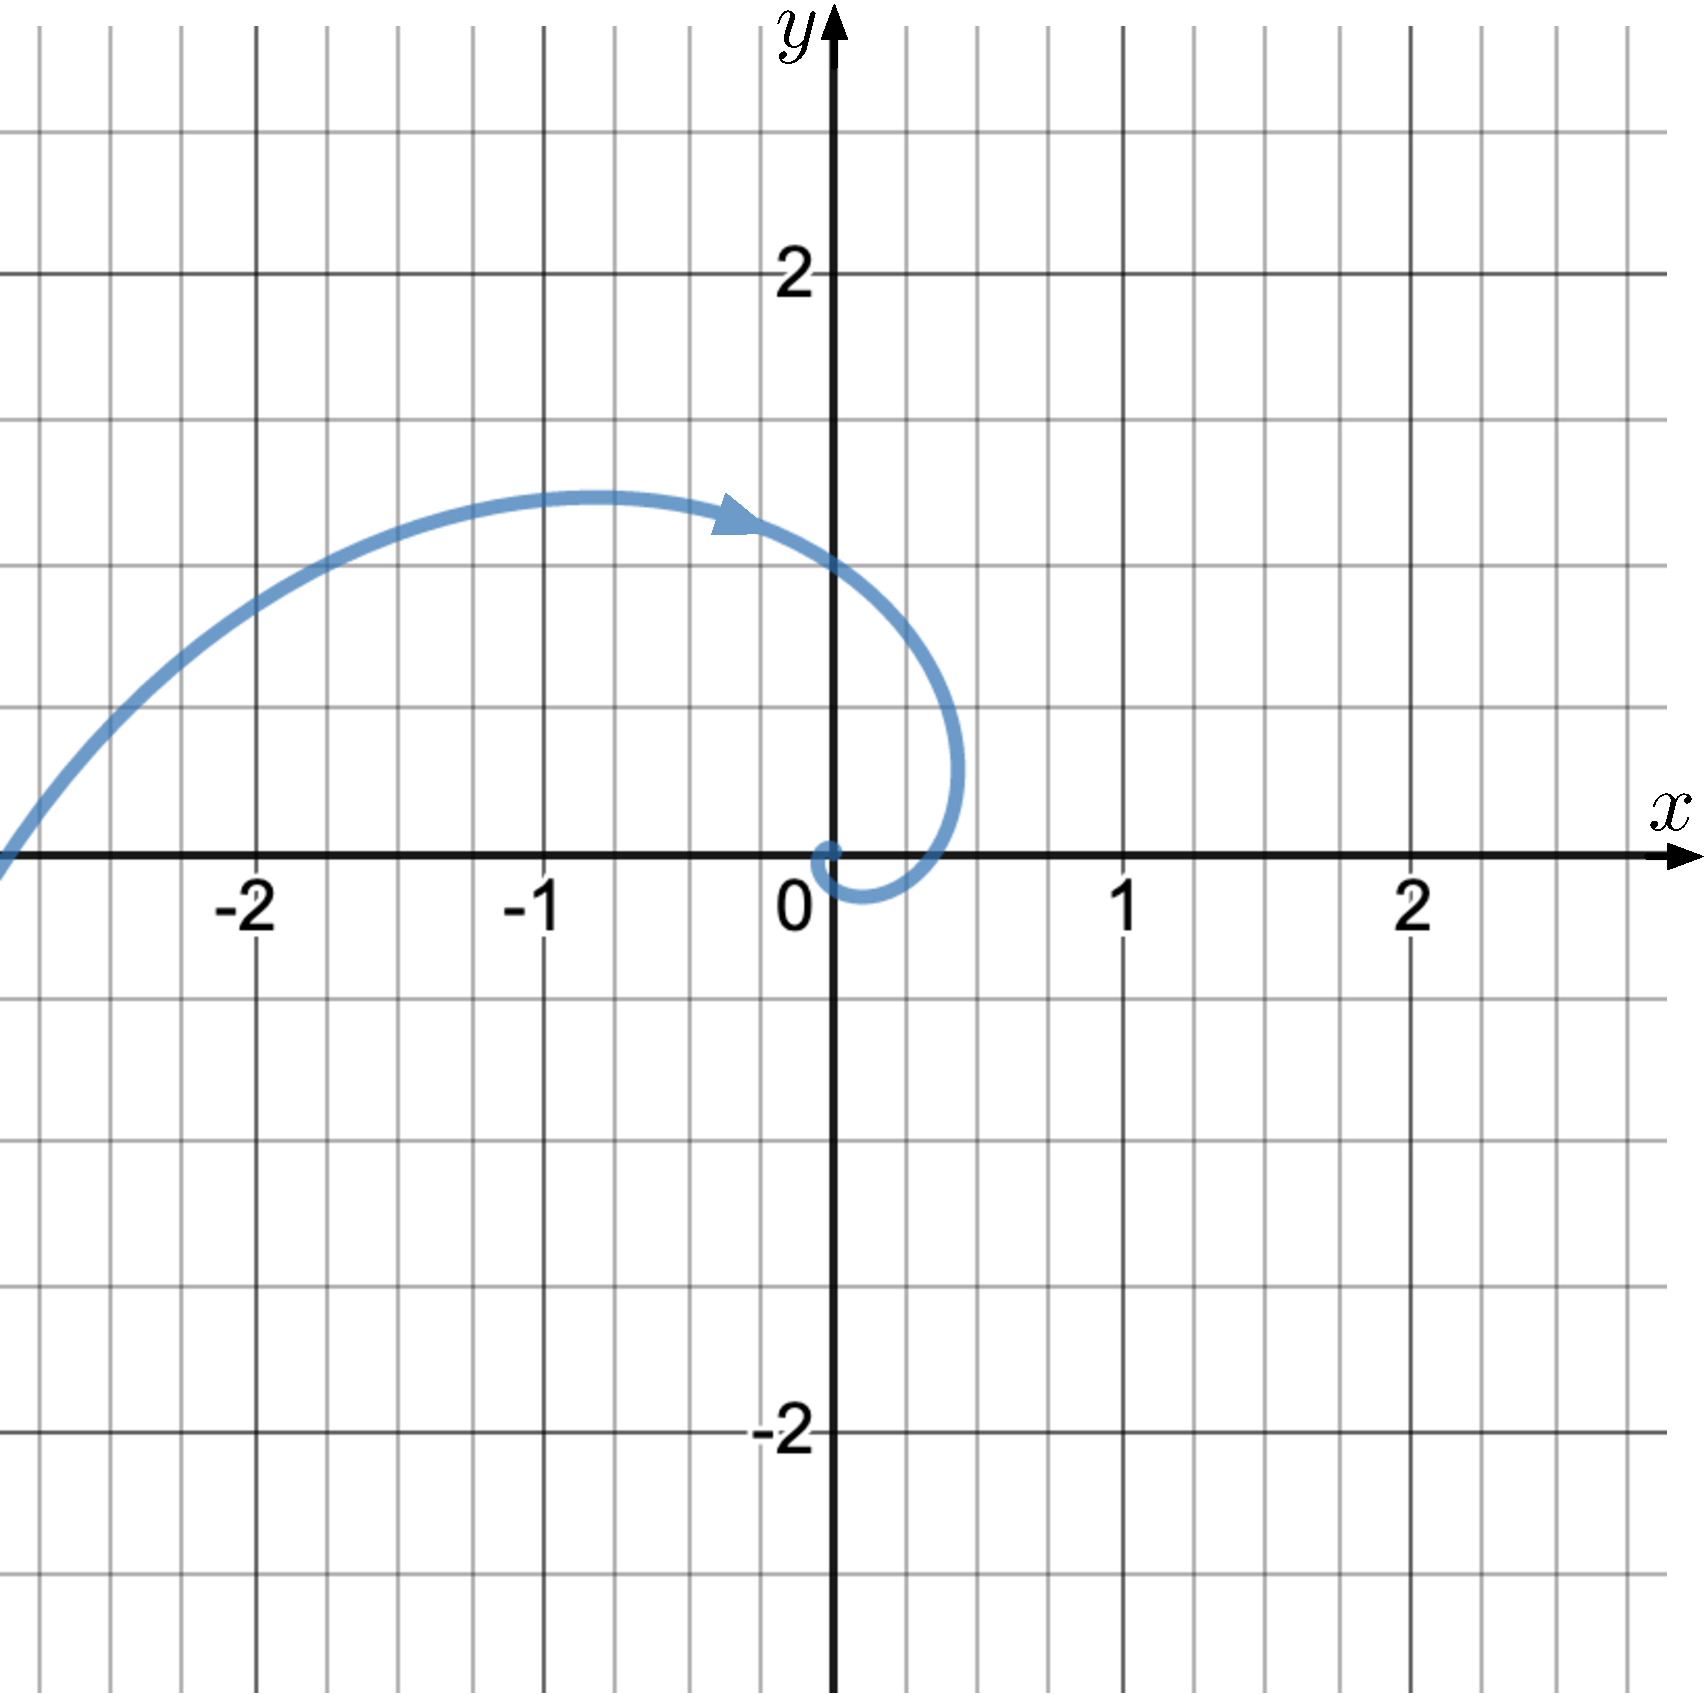
\includegraphics[height=200pt]{images/module18-spiral.pdf}
	\end{center}
	
	In this graph, we also include the graph for $t<0$. \\
	
	\item Let $c_1=-1$ and $c_2=0$ and we obtain
	$$ \vec{r}(t) = \begin{bmatrix}	 -\sin(3t) \\ -\cos(3t) \end{bmatrix} e^{-2t}$$	
	
	We add this graph to the previous one.
	\begin{center}
		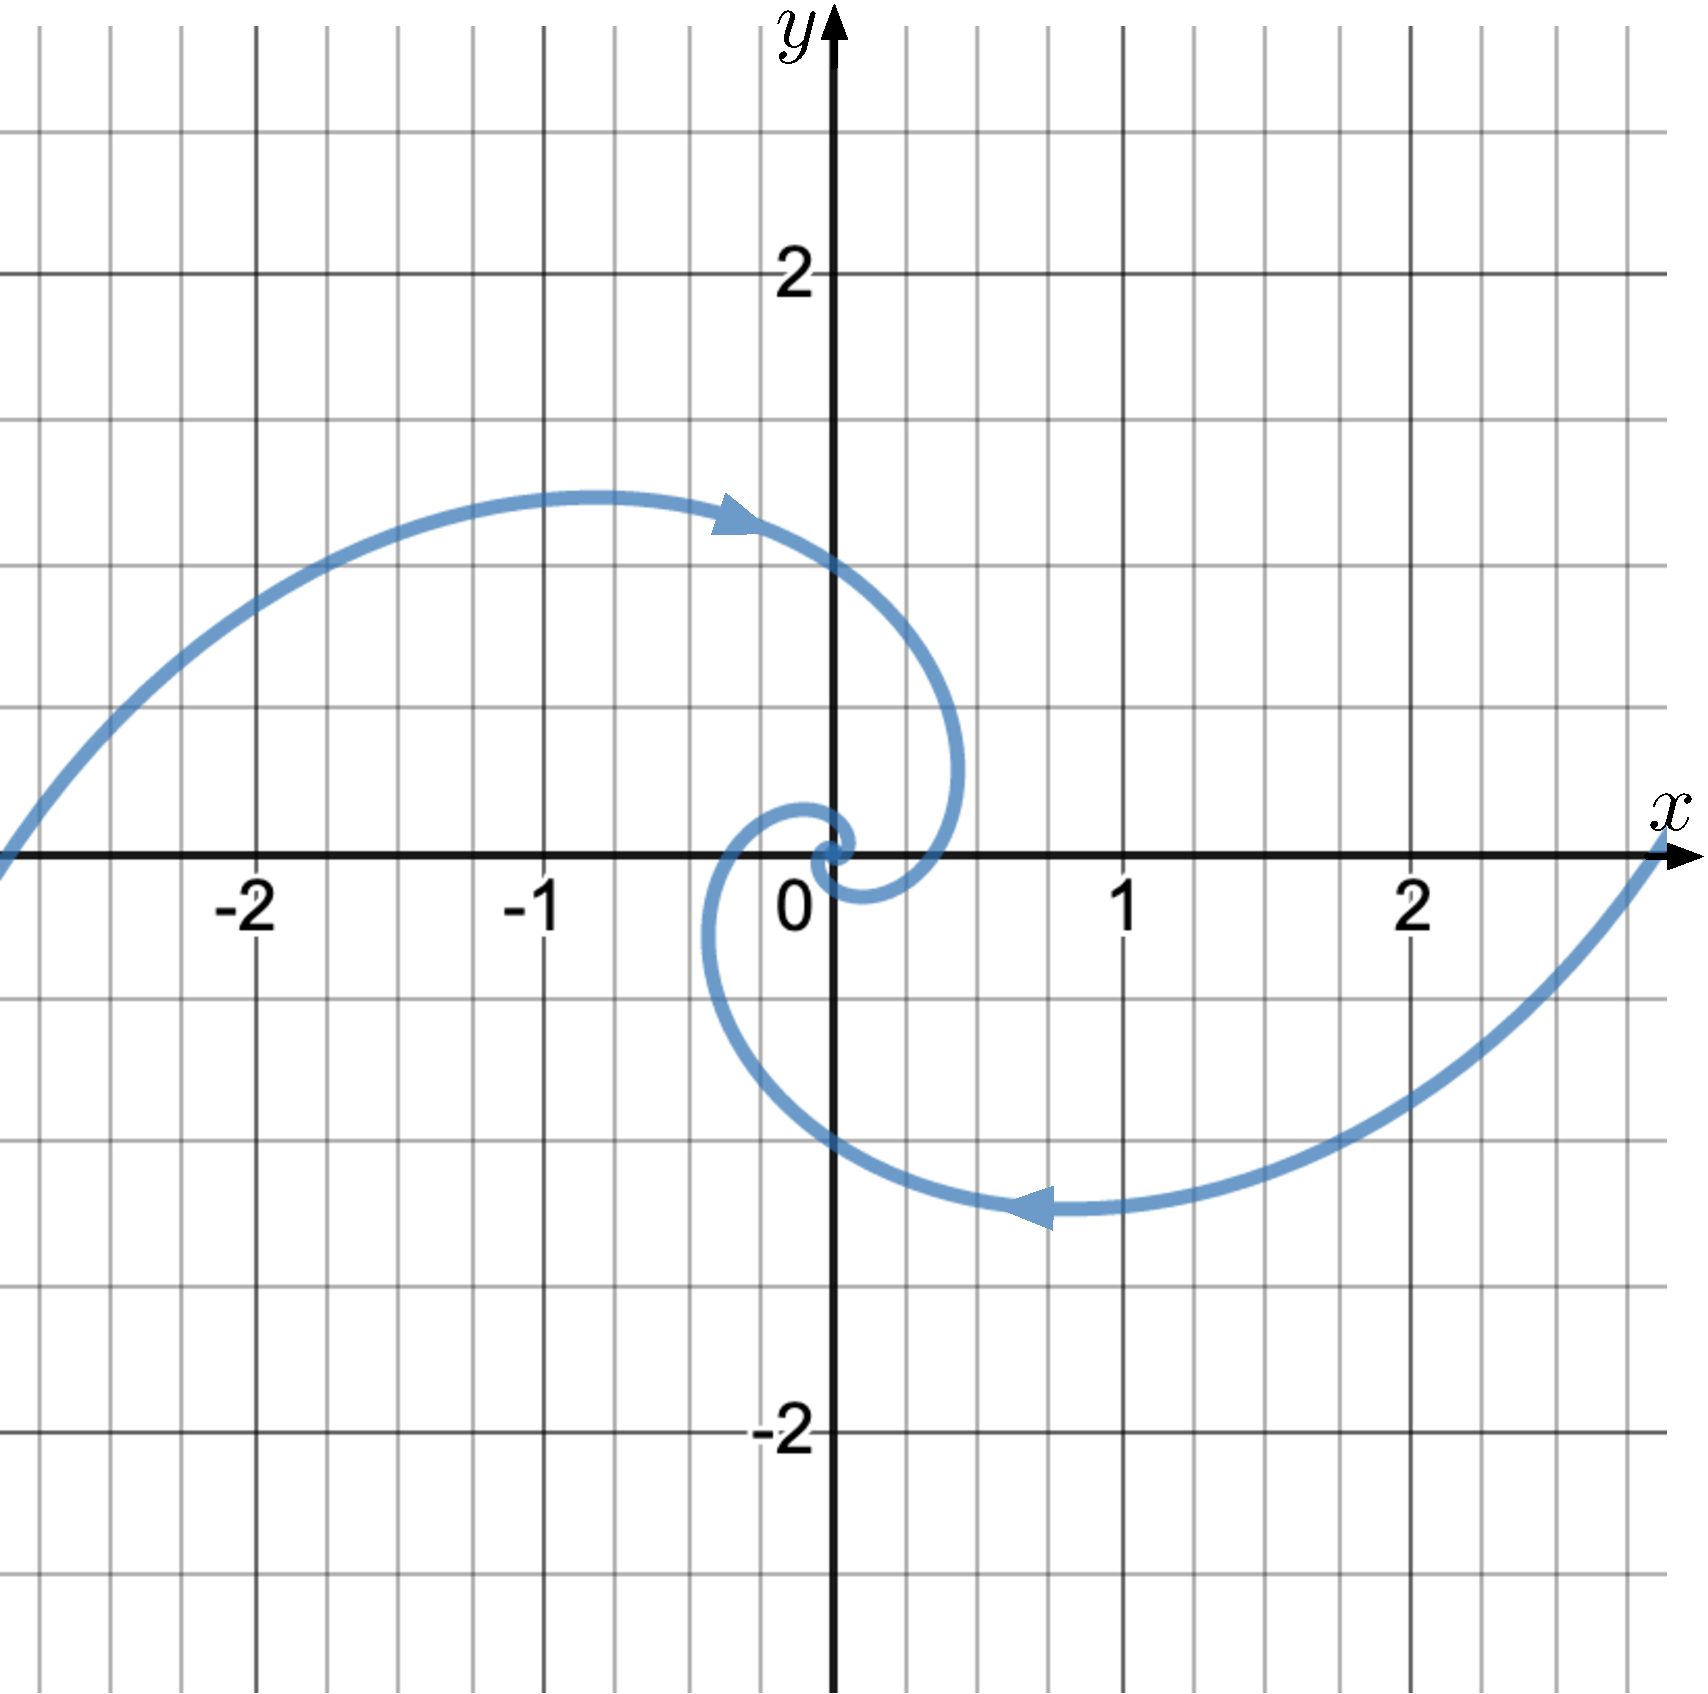
\includegraphics[height=200pt]{images/module18-spiral2.pdf}
	\end{center}
	
	\item Let $c_1=0$ and $c_2=\pm 1$ and we obtain
	$$ \vec{r}(t) = \begin{bmatrix}	 \mp \cos(3t) \\ \pm\sin(3t) \end{bmatrix} e^{-2t}.$$

	And add these to the graph:
	\begin{center}
		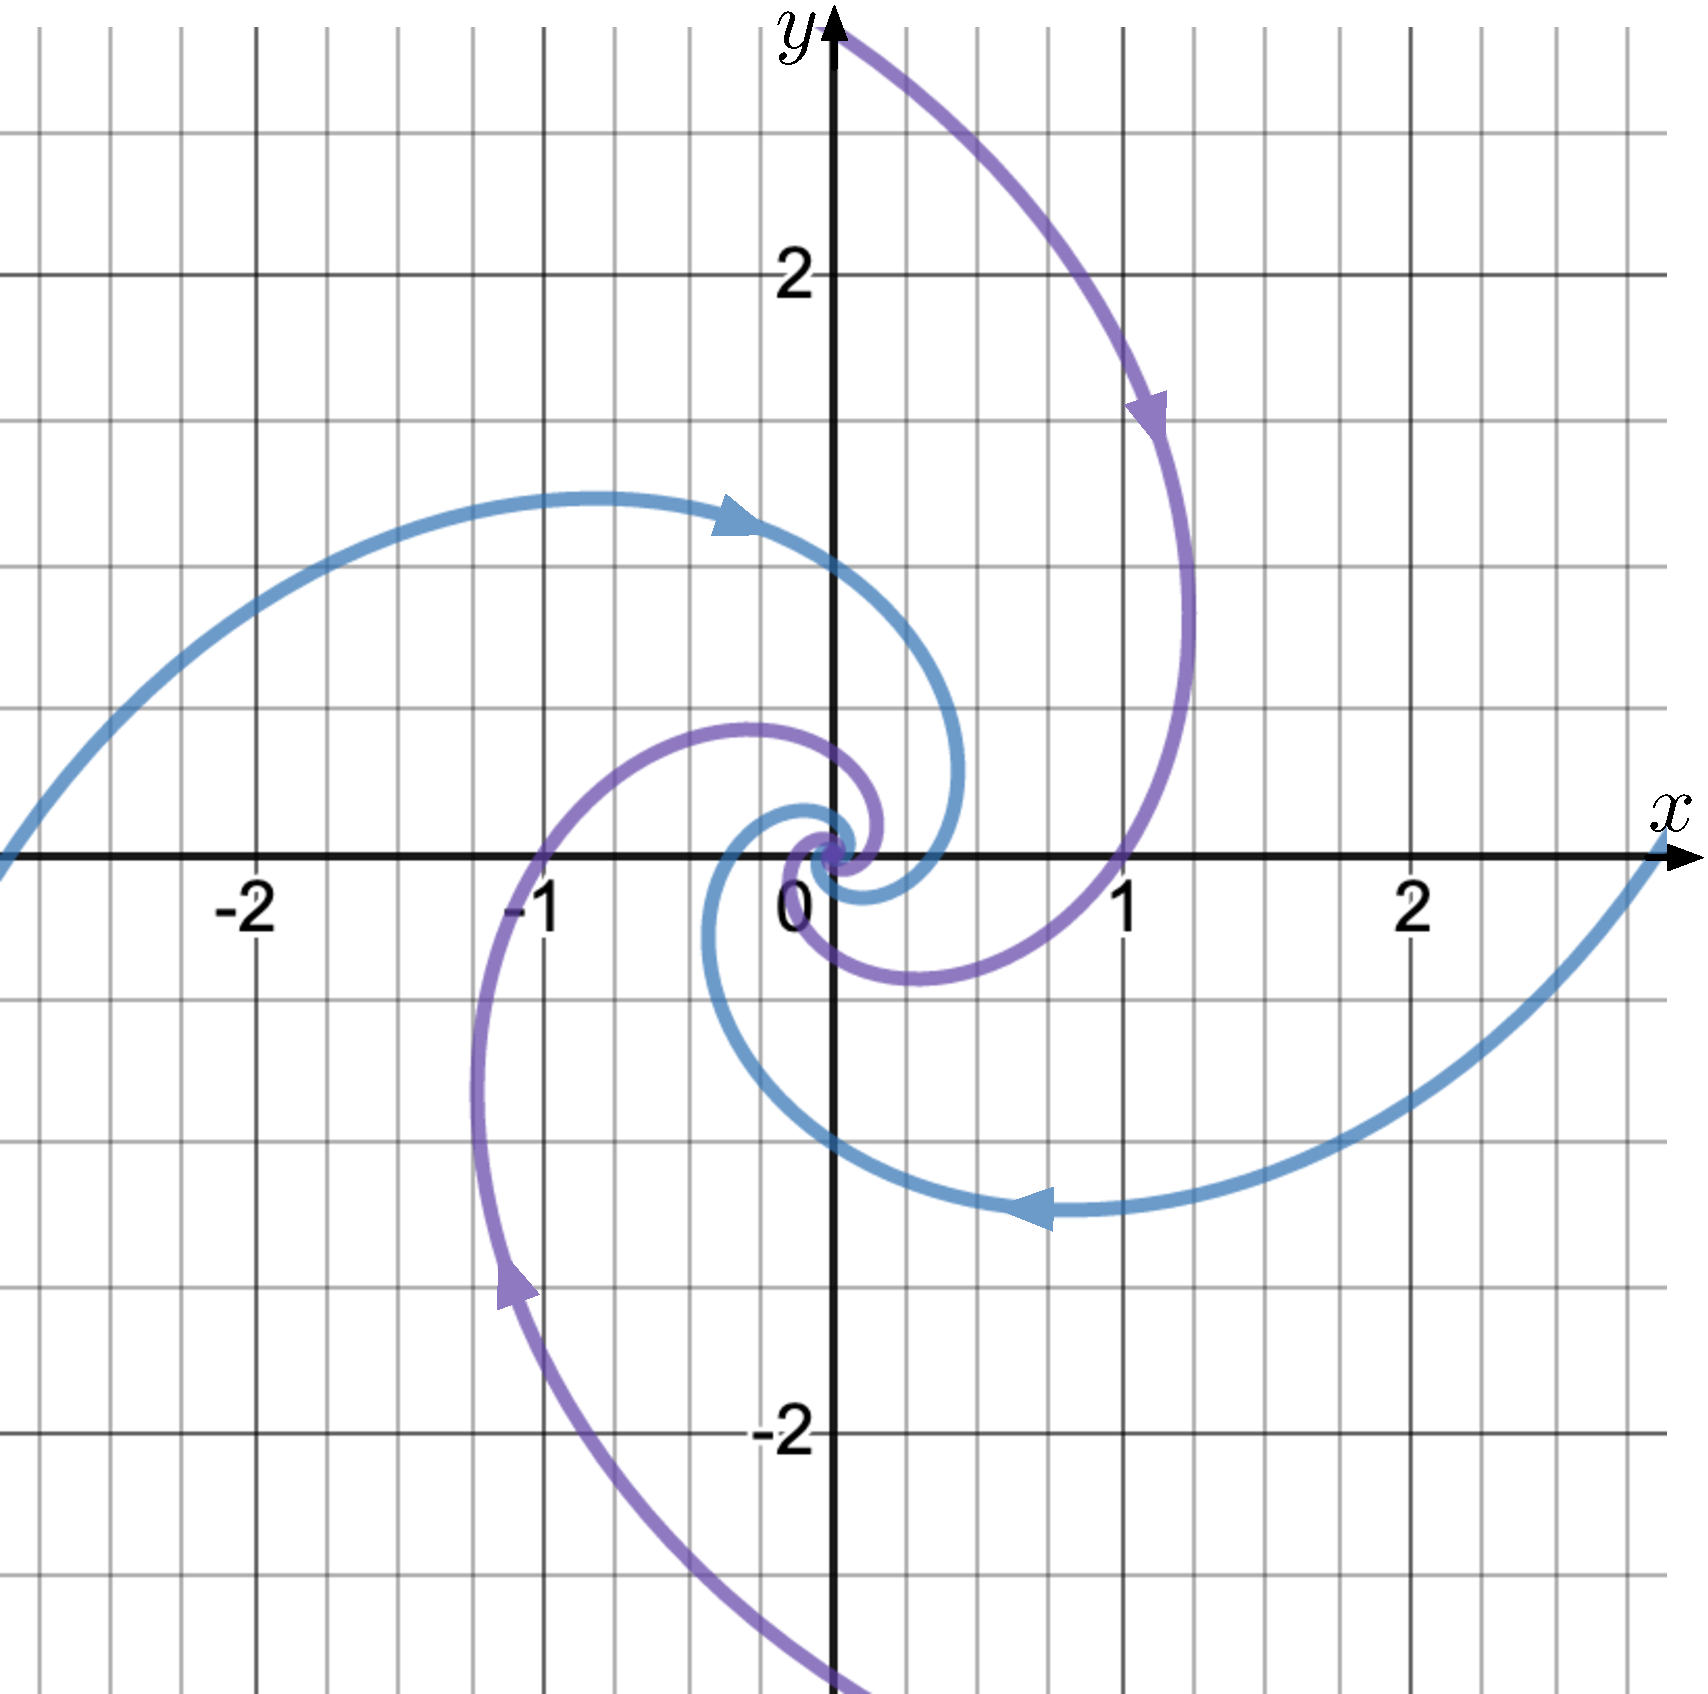
\includegraphics[height=200pt]{images/module18-spiral3.pdf}
	\end{center}

\end{itemize}

Sometimes, we need some solutions of the type $c_1=\pm 1$ and $c_2=\pm 1$ to get some different types of solutions, but we'll let you discover that on the core exercises.

These four solutions seem to give a good idea of all possible solutions: clockwise spirals converging to the origin.\\


Also observe that $\vec{r}(t) = \begin{bmatrix}0 \\ 0\end{bmatrix}$, so this system has an equilibrium solution.

This kind of equilibrium is called a \emph{spiral sink} and it is \emph{asymptotically stable}.
This means that it is a spiral and it converges to the equilibrium (the origin).
\end{example}





\begin{video}
	\begin{itemize}
		\item \qrvideo{https://youtu.be/nyI_JPDrJ_I}
		\item \qrvideo{https://youtu.be/dpbRUQ-5YWc}
	\end{itemize}
\end{video}





	\begin{exercises}

	\begin{problist}
	\prob For each matrix from practice problem \ref{mod16-gensol} from Module 16, sketch its phase portrait and label them as asymptotically stable or unstable. The system of ODEs is $\vec{r}'(t) = A \vec{r}(t)$ for the following matrices:
	\begin{enumerate}
	\begin{minipage}{.2\textwidth}
		\item $A = \begin{bmatrix} -7 & 6 \\ -9 & 8 \end{bmatrix}$;
		\item $A = \begin{bmatrix} 22 & 24 \\ -15 & -16\end{bmatrix}$;
		\item $A = \begin{bmatrix} 0 & 1 \\ -5 & 0 \end{bmatrix}$
		
		This is called a centre, which is stable, but not asymptotically stable. Can you tell why?
		\item $A = \begin{bmatrix} 0 & 1 \\ 5 & 0 \end{bmatrix}$;
		\item $A = \begin{bmatrix} 1 & \sqrt{3} \\ \sqrt{3} & -1\end{bmatrix}$;
		\item $A = \begin{bmatrix} 1 & \sqrt{3} \\ -\sqrt{3} & 1\end{bmatrix}$;
	\end{minipage}
	\qquad
	\begin{minipage}{.2\textwidth}
		\item $A = \begin{bmatrix} 0 & 1 \\ -4 & -4 \end{bmatrix}$
		
		This is called an improper node.
		\item $A = \begin{bmatrix} -4 & -6 \\ 2 & 3 \end{bmatrix}$;
		\item $A = \begin{bmatrix} 2 & -3 \\ 0 & 2 \end{bmatrix}$;
		\item $A = \begin{bmatrix} 2 & 0 \\ 0 & 2 \end{bmatrix}$;
		
		This is called a proper node.
		\item $A = \begin{bmatrix} 0 & 0 \\ 1 & 0\end{bmatrix}$; 
		\item $A = \begin{bmatrix} 0 & 0 \\ 0 & 1\end{bmatrix}$; 
	\end{minipage}
	\end{enumerate}
	
	\prob Consider a system of ODEs $\vec{r}'(t) = A \vec{r}(t)$.
	For each part, give an example of eigenvalues and eigenvectors of $A$ that would yield the required phase portrait:
	\begin{enumerate}
		\item Spiral sink (asymptotically stable);
		\item Spiral source (unstable);
		\item Centre (stable);
		\item Sink node (asymptotically stable);
		\item Source node (unstable);
		\item Saddle point (unstable);
		\item Improper node (stable);
		\item Improper node (unstable);
		\item Proper node (stable);
		\item Proper node (unstable);
	\end{enumerate}
	
	\prob Consider the system of ODEs
	$$
	\vec{r}'(t) = 
	\begin{bmatrix}
	1 & 1 \\ k & 1
	\end{bmatrix}\vec{r}(t).
	$$

	This system of ODEs changes behaviour depending on the parameter $k$.
	\begin{enumerate}
		\item Label the behaviour of the system for different values of $k$.
		\item We call the $k^\star$ the critical value of $k$ when the behaviour is different for $k<k^\star$ and for $k>k^\star$. For the critical value of $k$, sketch the phase portrait.
	\end{enumerate}
	
	
	\prob Consider the system of ODEs
	$$
	\vec{r}'(t) = 
	\begin{bmatrix}
	0 & 1 \\ -4 & -k
	\end{bmatrix}\vec{r}(t).
	$$

	This system of ODEs changes behaviour depending on the parameter $k$.
	\begin{enumerate}
		\item Label the behaviour of the system for different values of $k$.
		\item We call the $k^\star$ the critical value of $k$ when the behaviour is different for $k<k^\star$ and for $k>k^\star$. For the critical value of $k$, sketch the phase portrait.
		\item Which kinds of behaviours could be critical values?
	\end{enumerate}
	
	
	
	\prob Consider the system of ODEs
	$$
	\vec{r}'(t) = A \vec{r}(t).
	$$
	
	Let $T={\rm trace}(A) = a_{11}+a_{22}$, $D=\det(A) = a_{11}a_{22} - a_{12}a_{21}$, and $\Delta = T^2-4D$.
	
	\begin{enumerate}
		\item Show that the equilibrium solution is a saddle point if $D<0$.
		\item Show that the equilibrium solution is a spiral if $\Delta<0$ and $T\neq 0$.
		\item Show that the equilibrium solution is a centre if $T=0$ and $D>0$.
		\item When is the equilibrium point a node? \\

		\item Show that the equilibrium solution is asymptotically stable if $T<0$ and $D>0$.
		\item Show that the equilibrium solution is unstable if $T>0$ and $D<0$.
	\end{enumerate}






	\end{problist}
\end{exercises}

\end{module}



\begin{lesson}
	\Title{Phase Portraits}

	\Heading{Objectives}
	\begin{itemize}
		\item Bla
	\end{itemize}
	
	\Heading{Motivation} 

\end{lesson}





\question
	Consider the following model for cheetah's and lions, where
	$$ \vec{p}(t) = \begin{bmatrix} \ell(t) = \text{population of lions} \\ c(t) = \text{population of cheetahs} \end{bmatrix} $$
	which satisfies
	$$
	\frac{d\,\vec{p}}{dt} = \begin{bmatrix}
 		1 & -1 \\
 		-3 & 1
 	\end{bmatrix}
	$$
	
	The general solution is:
	$$
	\vec{p}(t) = c_1 \begin{bmatrix} 1 \\ \sqrt{3} \end{bmatrix} e^{(1-\sqrt{3})t} + c_2 \begin{bmatrix} -1 \\ \sqrt{3} \end{bmatrix} e^{(1+\sqrt{3})t}.
	$$
\begin{parts}
	\item Without computing them, what are the eigenvalues and eigenvectors of the matrix?
	\item Sketch the graph of the solution with $c_1=\pm 1$ and $c_2=0$.
	\item Sketch the graph of the solution with $c_1=0$ and $c_2=\pm 1$.
	\item When one constant is set to 0, what is the shape of the graph? Is it always like that? Can you prove it?
	\item Sketch the graph of the solution with $c_1=\pm 1$ and $c_2=\pm 1$.
	\item Provide an interpretation of the different types of solutions.
\end{parts}

\begin{annotation}
	\begin{goals}
	At the end, let the students know that the equilibrium is called \emph{saddle point} and it is \emph{unstable}, because solutions go away from it.
	
	For the interpretation question, when one population hits zero, it is extinct, so the graph doesn't make sense. 
	
	We can interpret that if a population becomes extinct, then the other will behave as it would without competitors: grow exponentially fast!
	\end{goals}
\end{annotation}






\bookonlynewpage

\question
	Let us expand the model from the previous exercise to:
	$$ \vec{p}(t) = \begin{bmatrix} \ell(t) = \text{population of lions} \\ c(t) = \text{population of cheetahs} \end{bmatrix} $$
	which satisfies
	$$
	\frac{d\,\vec{p}}{dt} = \begin{bmatrix}
 		1 & -1 \\
 		-3 & 1
 	\end{bmatrix} \vec{p}
 	+ \begin{bmatrix}
 		- 10 \\ 50
	 \end{bmatrix} \vec{p}.
	$$
	
	The extra term corresponds to the effect of harvesting 10 lions and bringing in 50 cheetahs every year to the reserve. \\
	
	The general solution is:
	$$
	\vec{p}(t) = \begin{bmatrix} 20 \\ 10 \end{bmatrix} +
		c_1 \begin{bmatrix} 1 \\ \sqrt{3} \end{bmatrix} e^{(1-\sqrt{3})t} + c_2 \begin{bmatrix} -1 \\ \sqrt{3} \end{bmatrix} e^{(1+\sqrt{3})t}.
	$$
\begin{parts}
	\item Sketch the phase portrait.
	\item Provide an interpretation of the different types of solutions.
\end{parts}

\begin{annotation}
	\begin{goals}
		Some students might try to sketch everything from scratch.
		Remind them that the solutions look very similar and they only have to adapt the phase portrait they had before.
	\end{goals}
\end{annotation}



\bookonlynewpage


\question
	For each of the following general solutions, sketch the phase portrait.
\begin{parts}
	\item $	\vec{r}(t) = c_1 \begin{bmatrix} 2 \\ 1 \end{bmatrix} e^{2t} + c_2 \begin{bmatrix} -1 \\ 1 \end{bmatrix} e^{5t}.$
	\item $	\vec{r}(t) = c_1 \begin{bmatrix} 2 \\ 1 \end{bmatrix} e^{-2t} + c_2 \begin{bmatrix} -1 \\ 1 \end{bmatrix} e^{-5t}.$	
\end{parts}
\begin{annotation}
	\begin{goals}
	At the end, let the students know that these equilibria are called 
	\begin{itemize}
		\item \emph{source} and it is \emph{unstable}, because solutions go away from it.
		\item \emph{sink} and it is \emph{asymptotically stable}, because solutions converge to it.
	\end{itemize}
	
	If there is time, students can think about:

	Given a matrix $A$, which part of $A$ indicates whether the equilibrium is stable / unstable? Which part indicates whether it's a sink/source vs spiral sink/source?
	\end{goals}
\end{annotation}





\standardonlynewpage

%%%%%%%%%%%%%%%%%%%%%%%%%%%%%%
%
%  MODULE - Analysis of Systems
%
%%%%%%%%%%%%%%%%%%%%%%%%%%%%%%



\begin{module}{Analysis of Models with Systems}
	\label{sys:analysis}

	In this module you will learn
\begin{itemize}
	\item different ways to analyze models with several differential equations
\end{itemize}

\hfill \\



In this chapter, we have learned how to create models involving systems of ODEs and how to solve some special types of systems of ODEs.

Once we create a model that involves a system of ODEs, the ultimate goal is not to solve the system of ODEs, but to be able to understand how the situation will develop.
Solving the system of ODEs is often a large step in that direction, but it is more important to know how to interpret it in light of the original situation.

Sometimes, when we cannot find an explicit formula for the solution, it is still possible to study the system to find some properties and behaviours of the solutions. \\

In this module, we'll study one example using a few different methods.


\begin{example}
The goal here is not the modelling but the analysis of the model, so we will quickly explain the model. \\

We are going to model population versus cost of living in Toronto.


Consider the following functions
\begin{itemize}
\item $p(t) = $ Population of Toronto (GTA) in millions, $t$ years since the beginning of 2015.
\item $c(t) = $ Cost of living in Toronto (in thousands of dollars), $t$ years since the beginning of 2015.
\item Define a vector $\vec{x}(t) = \begin{bmatrix} p(t) \\ c(t) \end{bmatrix}$.
\end{itemize}

We assume that these two factors are related according to the following properties:
\begin{itemize}
\item In the absence of any migration, the population will decrease proportionally to the cost of living (with constant $a$);
\item There are always people moving into Toronto independently of its current population or cost of living (with constant $b$)
\item In the absence of any other factors, the cost of living; increases proportionally to the population (with constant $d$)
\item In the absence of any other factors, the cost of living; increases proportionally to the cost of living due to inflation (with constant $e$);
\item The city is always expanding, so the cost of living is always decreasing independently of its current population or cost of living (with constant $f$).
\end{itemize}
The constants $a,b,d,e,f$ are all positive. \\

Our model is:
$$
\vec{x}'(t) = 
	\begin{bmatrix}
 		0 & -a \\
 		d & e
	\end{bmatrix}
					\vec{x}(t) + 
	\begin{bmatrix}
		b \\ -f
	\end{bmatrix}
$$
\end{example}

\hfill

\begin{center}
\textbf{\color{cyan}
Qualitative evolution of quantities
}
\end{center}


%\paragraph{Qualitative evolution of quantities.}
We can try to figure out how these quantities, $p(t)$ and $c(t)$, are going to increase or decrease. \\

As an academic example, let us imagine that initially  \quad $p(0)=c(0)=0$.

Then, at $t=0$, we have
$$
p'(0)= b > 0 \quad \text{ and } \quad
c'(0)=-f < 0.
$$

This means that $p(t)$ is increasing while $c(t)$ wants to decrease.

Here we need to make sure that everything still makes sense: since it doesn't make sense to have a negative cost of living (government incentives to move into the city?!), we need to disregard our system and assume that $c(t)$ will continue constant while $c'(t)<0$.

We then have:
\begin{graybox}
\begin{center}
\begin{tabular}{c||c|c|c|c|c|c|c|c}
$\pmb{t}$	& $0$ 		& 			& &  			& 			& 	&	& \hspace{1cm} $+\infty$ \\[5pt] \hline\hline
$\pmb{p}$ & $0$	& $\nearrow$	& \hspace{0.5cm} &	\hspace{1cm}	&	&  \hspace{0.5cm}	&  	& 	\\[5pt] \hline
$\pmb{c}$ & $0$		& $\rightarrow$	&  0 & \hspace{1cm} & 	\hspace{0.5cm}	& \hspace{1cm} 	& \hspace{0.5cm}	&\hspace{1cm}	\\[5pt]
\end{tabular}
\end{center}
\end{graybox}

While $c(t)=0$, we have
$$
p'(t)= b > 0  \quad \text{ and } \quad 
c'(t)=d\, p(t) -f.
$$

This means that $p(t)$ is increasing with constant slope (linearly) until $c'(t_1)=0$.
We can figure out when this will happen:
$$
0=c'(t_1)=d\, p(t_1) -f \quad \Leftrightarrow \quad p(t_1) = \frac{f}{d}.
$$

So we continue our table:
\begin{graybox}
\begin{center}
\begin{tabular}{c||c|c|c|c|c|c|c|c}
$\pmb{t}$	& $0$ 		& 			& $t_1$ &  			& 			& 	&	& \hspace{1cm} $+\infty$ \\[5pt] \hline\hline
$\pmb{p}$ & $0$	& $\nearrow$	& $\displaystyle\frac{f}{d}$ &	\hspace{1cm}	&	&  \hspace{0.5cm}	&  	& 	\\[5pt] \hline
$\pmb{c}$ & $0$		& $\rightarrow$	&  0 & \hspace{1cm} & 	\hspace{0.5cm}	& \hspace{1cm} 	& \hspace{0.5cm}	&\hspace{1cm}	\\[5pt]
\end{tabular}
\end{center}
\end{graybox}

What happens after $t_1$?

Consider $t>t_1$ slightly after $t_1$. Then
$$
\begin{cases}
p'(t) = -a c(t) + b >0 & \text{ still positive because $c(t)$ is very small, but the slope is decreasing} \\
c'(t) = d p(t) + e c(t) - f	>0 & \text{ increasing quickly as both $p$ and $c$ increase}
\end{cases}
$$

\begin{graybox}
\begin{center}
\begin{tabular}{c||c|c|c|c|c|c|c|c}
$\pmb{t}$	& $0$ 		& 			& $t_1$ &  			& 			& 	&	& \hspace{1cm} $+\infty$ \\[5pt] \hline\hline
$\pmb{p}$ & $0$	& $\nearrow$	& $\displaystyle\frac{f}{d}$ &	\IncDown	&	&  \hspace{1cm}	&  	& 	\\[5pt] \hline
$\pmb{c}$ & $0$		& $\rightarrow$	&  0 & \IncUp & 	\hspace{0.5cm}	& \hspace{1cm} 	& \hspace{0.5cm}	&\hspace{1cm}	\\[5pt]
\end{tabular}
\end{center}
\end{graybox}

At a certain time $t_2$, the population will stop increasing. Let us find out when this happens:
$$
0=p'(t_2) = -a c(t_2) + b >0 
	\quad \Leftrightarrow \quad c(t_2) = \frac{b}{a}.
$$

\begin{graybox}
\begin{center}
\begin{tabular}{c||c|c|c|c|c|c|c|c}
$\pmb{t}$	& $0$ 		& 			& $t_1$ &  			& 	$t_2$		& 	&	& \hspace{1cm} $+\infty$ \\[5pt] \hline\hline
$\pmb{p}$ & $0$	& $\nearrow$	& $\displaystyle\frac{f}{d}$ &	\IncDown	& $\rightarrow$	&  \hspace{1cm}	&  	& 	\\[5pt] \hline
$\pmb{c}$ & $0$		& $\rightarrow$	&  0 & \IncUp & 	 $\displaystyle \frac{b}{a}$	& \hspace{1cm} 	& \hspace{0.5cm}	&\hspace{1cm}	\\[5pt]
\end{tabular}
\end{center}
\end{graybox}

After this point we have $t>t_2$ slightly after $t_2$:
$$
\begin{cases}
p'(t) = -a c(t) + b <0 & \text{ decreasing rapidly while $c'(t)>0$}\\
c'(t) = d p(t) + e c(t) - f	>0 & \text{ still increasing quickly until $p(t)=0$}
\end{cases}
$$

We expect that at some point $p(t_3)=0$. From that point on we have
$$
\begin{cases}
p'(t_3) = -a c(t_3) + b <0 & \text{ we need to ignore the model at this point and keep $p$ constant}\\
c'(t_3) = e c(t_3) - f	>0 & \text{ still increasing exponentially, as long as } c(t_3) > \frac{f}{e}
\end{cases}
$$

So this is our final table:
\begin{graybox}
\begin{center}
\begin{tabular}{c||c|c|c|c|c|c|c|c}
$\pmb{t}$	& $0$ 		& 			& $t_1$ &  			& 	$t_2$		& 	& $t_3$	& \hspace{1cm} $+\infty$ \\[5pt] \hline\hline
$\pmb{p}$ & $0$	& $\nearrow$	& $\displaystyle\frac{f}{d}$ &	\IncDown	& $\rightarrow$	&  \DecDown	& 0 	& $\rightarrow$	\\[5pt] \hline
$\pmb{c}$ & $0$		& $\rightarrow$	&  0 & \IncUp & 	 $\displaystyle \frac{b}{a}$	& \IncUp 	& 	& \IncUp	\\[5pt]
\end{tabular}
\end{center}
\end{graybox}



Observe that to do this analysis, we didn't need to know how to solve the system of ODEs. \\






\begin{center}
\textbf{\color{cyan}
Finding the equilibrium point(s)
}
\end{center}

%\paragraph{Finding the equilibrium point.} 
This is often easy to find, and by using the intuition we gained while learning to sketch phase portraits, this can give us a lot of insight about the solutions.

Let us find the equilibrium point:
$$
\begin{cases}
0= p'(t) = -a c(t) + b \\
0= c'(t) = d p(t) + e c(t) - f	
\end{cases}
\quad \Leftrightarrow \quad 
	\begin{cases}
 	\displaystyle c(t) = \frac{b}{a} \\[5pt]
	\displaystyle p(t) = \frac{af - be}{ad}
	\end{cases}
$$

Observe that if the population and cost of living are at these levels, then they will remain constant. \\

This also informs us that the disastrous scenario on the first analysis, where the population all left the city, might have been caused by the stating position. \\






\begin{center}
\textbf{\color{cyan}
Interpreting the phase portrait
}
\end{center}

We have seen in the last module how to sketch a phase portrait for a system of ODEs such as this one.

Let us assume that the constants $a=b=d=e=1$, $f=2$. Then the phase portrait is
\begin{center}
	\includegraphics*[width=250pt]{images/module18-pc.pdf}
\end{center}

Observe that both quantities should be positive, so let us focus on the quadrant where both are positive:
\begin{center}
	\includegraphics*[width=250pt]{images/module18-pc-closeup.pdf}
\end{center}

Observations:
\begin{itemize}
	\item Whenever a graph hits the axes, we must stop the model and re-evaluate what that means: when the graph hits the $c=0$ axis, then the population will start increasing until $c'>0 \Leftrightarrow p = 2$, so the graph will continue horizontally until the point $(2,0)$ where the model restarts.
	\item The population seems to converge to $0$ in all cases.
	\item The purple case seems to be an interesting one where the population and cost of living oscillate for a bit near the equilibrium and then the cost of living goes almost to zero before starting to go up again and forcing all the people to leave the city.
\end{itemize}



\hfill

\begin{center}
\textbf{\color{cyan}
Properties of the system
%Other questions about the system
}
\end{center}

%\paragraph{Other questions about the system.} 
We can look for other properties of the system of ODEs.

Based on the two analyses above, we can ask the following question:
\begin{itemize}
	\item Is there a value for the cost of living such that if it is above that, then eventually all the population will leave the city?
\end{itemize}

We know that 
$$
p'(t) = -a c(t) + b < 0 \quad \Leftrightarrow \quad c(t) > \frac{b}{a}.
$$

So as long as the cost of living is above $\frac{b}{a}$, then the population will continue to decrease. \\

Observe that depending on the constants $d, e, f$, we could still have
$$
c'(t) = d p(t) + e \frac{b}{a} - f < 0,
$$
so that we could end up with a cycle around the equilibrium we found before.









	\newpage 

\begin{exercises}

	\begin{problist}
	\prob Consider the model for student learning:
	\begin{itemize}
		\item $\vec{x} = \begin{bmatrix} x_1 \\ x_2 \end{bmatrix}$
		\item $x_1=$ student confidence in his/her own abilities ($x_1 \in [0,1]$)
		\item $x_2=$ student knowledge measured in IQ past 100
		\item $\vec{x}'(t) =
		\begin{bmatrix}
			a & b \\
			c & - d 
		\end{bmatrix}
		\vec{x}(t)
		+ \begin{bmatrix}
 			-e \\ 0
 		\end{bmatrix}$
		\item Constants $a,b,c,d,e>0$.
	\end{itemize}
	\begin{enumerate}
		\item What is the equilibrium solution $\vec{x}_e$? 
		\item If tests are harder, then $d$ is larger. How does that affect the equilibrium confidence and knowledge of students?
		\item Is the equilibrium solution stable?
		\item Assume $a=1, b=c=2, d=3,e=0$. As $t \to +\infty$, what are the possible outcomes for $\vec{x}(t)$ Explain the meaning for the students.
		\item Assume $a=1, b=c=2, d=3,e=0$. Some solutions satisfy $\displaystyle \lim_{t \to +\infty} \begin{bmatrix}c(t) \\ k(t) \end{bmatrix} = \begin{bmatrix} + \infty \\ + \infty \end{bmatrix}$.

			Show on a graph which initial conditions $\vec{x}(0) = \begin{bmatrix}c(0) \\ k(0) \end{bmatrix}$ guarantee this limit?

		\item If the tests become harder, i.e., $d$ increases, then is that good or bad for students?.
	\end{enumerate}
	
	\prob Consider the model for a tree:
	\begin{itemize}
		\item $\vec{x}(t) = \begin{bmatrix} \ell(t) \\ h(t) \end{bmatrix}$
		\item $\ell(t)=$ area of leafs on the tree
		\item $h(t)=$ height of the tree
		\item $\vec{x}'(t) =
		\begin{bmatrix}
			a & -b \\
			c & -d 
		\end{bmatrix}
		\vec{x}(t)$
		\item Constants $a,b,c,d>0$.
	\end{itemize}
	\begin{enumerate}
		\item Is it possible to have the tree growing taller and taller forever while the leaf area remains bounded?
		\item What would happen to the tree if the area of leafs is proportional to the height squared (not square root)?
		\item If $ad=bc$, explain what happens to the tree as $t\to \infty$.
	\end{enumerate}
	
	
	\prob Consider the model of a car:
	\begin{itemize}
		\item $\vec{c}(t) = \begin{bmatrix} v(t) \\ f(t) \end{bmatrix}$
		\item $v(t)=$ speed of the car
		\item $f(t)=$ amount of fuel in the car's tank
		\item $\vec{c}'(t) =
		\begin{bmatrix}
			-2 & 1 \\
			-2 & 0 
		\end{bmatrix}
		\vec{c}(t)
		+ \begin{bmatrix}
 			0 \\ -1	
		\end{bmatrix}$
	\end{itemize}
	\begin{enumerate}
		\item What is the equilibrium solution $\vec{c}_{\rm eq}$? What is the meaning of your result?
		\item If the car runs out of fuel at 300 m/s, then describe what happens to the car. 
		\item Describe what happens to the car when it starts at rest with a full tank of $300$ L.
		\item If the car attains its maximum velocity when there are still $300$ L of fuel left, what was the car's maximum velocity?


	\end{enumerate}


	\prob Consider the model for crying babies:
	\begin{itemize}
		\item $\vec{c}(t) = \begin{bmatrix} a(t) \\ b(t) \end{bmatrix}$
		\item $a(t)=$ volume of baby A's cries in dB
		\item $b(t)=$ volume of baby B's cries in dB
		\item $\vec{c}'(t) =
		\begin{bmatrix}
			-\alpha & \beta \\
			\beta & -\alpha 
		\end{bmatrix}
		\vec{c}(t)$
		\item constants $\alpha,\beta>0$.
	\end{itemize}

	The constants $\alpha$ and $\beta$ are $1$ and $2$. Does it make a difference which is 1 and which is 2?


	
		
	\end{problist}
\end{exercises}
\end{module}



\begin{lesson}
	\Title{Analysis of Models with Systems}
%
%	\Heading{Objectives}
%	\begin{itemize}
%		\item Bla
%	\end{itemize}
%	
%	\Heading{Motivation} 

\end{lesson}




\question
	Consider the following model for the sales from a designer clothing brand:
	\begin{itemize}
	\item $x_1(t) = $ purchases by ``common mortals'' (CM) at time $t$ in years since the beginning of 2015.
	\item $x_2(t) = $ purchases by ``famous people'' (FP) at time $t$.
	\end{itemize}
	
	Our model is based on the following two principles:
	\begin{enumerate}[label={($P_{\arabic*}$)}]
		\item CM will buy more items from the brand when CM or FP buy more.
		\item FP will buy less when CM buy them, but will buy more when FP buy it.
	\end{enumerate}

	The model we considered is:
	$$
	\vec{x}'(t) = 
	\begin{bmatrix}
 		a & b \\
 		-c & d
	\end{bmatrix}
	\vec{x}(t)
	$$
	
	\begin{parts}
		\item Suppose that at the beginning only CM buy this brand. Describe how $x_1(t)$ and $x_2(t)$ evolve as $t>0$.


		\item Suppose that at the beginning only FP buy this brand. Describe how $x_1(t)$ and $x_2(t)$ evolve as $t>0$.


		\item What conditions on the constants $a,b,c,d$ will guarantee that the solutions will spiral? In that case, is it a spiral source or spiral sink? Is it clockwise or counterclockwise?
		\item Are there constants $a,b,c,d>0$, such that the solution $\vec{x}$ is periodic?
		\item Consider the constants $a=b=c=d=1$. Assume that initially CM were buying $c_0>0$ items and FP were buying $f_0>0$ items.
			What will happen to $x_1(t)$ and $x_2(t)$ as $t \to \infty$? Explain the results in terms of the evolution of purchases from CM and FP.
		\item Consider the constants $a=b=c=d=1$.  If $c_0=10$, $f_0=100$, then at what time will FP stop buying items? And at what time will FP be buying the maximum number of items?
	
	\end{parts}




\bookonlynewpage


\hfill

\bookonlynewpage
\standardonlynewpage
